\documentclass[12pt,a4paper]{article}
\usepackage[utf8]{inputenc}
\usepackage[vietnamese]{babel}
\usepackage{fancyhdr}
\usepackage{amsmath}
%\usepackage[utf8]{vietnam}
\usepackage{amsfonts}
\usepackage{xcolor}
\usepackage{longfbox}
\usepackage{titlesec}
\usepackage{enumitem}
\usepackage{mdframed}
\usepackage{amssymb}
\usepackage{pgf,tikz,pgfplots}
\usepackage{graphicx}
\graphicspath{ {figures/} {photo/} {./} }
\usepackage{array}
\usepackage{cases}
\usepackage{listings}
\usepackage{color}
\usepackage{float} 
\usepackage{array, caption, tabularx,  ragged2e,  booktabs}
\usepackage{hyperref}
\usepackage{tabulary}
\usepackage{algorithm}
\usepackage{algpseudocode}
\usepackage{longtable}
\usepackage{multirow}
\usepackage{subcaption}
\pgfplotsset{compat=1.5}
\usepackage{mathrsfs}
\usetikzlibrary{arrows, calc, positioning, shapes.geometric, shapes.misc}
\usepackage{fancyhdr}
\pagestyle{fancy}
\usepackage[labelsep=endash]{caption}
\pagestyle{empty}

% Code listing colors
\definecolor{dkgreen}{rgb}{0,0.6,0}
\definecolor{gray}{rgb}{0.5,0.5,0.5}
\definecolor{mauve}{rgb}{0.58,0,0.82}
\definecolor{codegreen}{rgb}{0,0.6,0}
\definecolor{codegray}{rgb}{0.5,0.5,0.5}
\definecolor{codepurple}{rgb}{0.58,0,0.82}
\definecolor{backcolour}{rgb}{0.95,0.95,0.92}

% Code listing style
\lstdefinestyle{mystyle}{
    backgroundcolor=\color{backcolour},   
    commentstyle=\color{codegreen},
    keywordstyle=\color{magenta},
    numberstyle=\tiny\color{codegray},
    stringstyle=\color{codepurple},
    basicstyle=\ttfamily\footnotesize,
    breakatwhitespace=false,         
    breaklines=true,                 
    captionpos=b,                    
    keepspaces=true,                 
    numbers=left,                    
    numbersep=5pt,                  
    showspaces=false,                
    showstringspaces=false,
    showtabs=false,                  
    tabsize=2,
    frame=single,
    aboveskip=3mm,
    belowskip=3mm,
}
\lstset{style=mystyle}

% Language definitions for listings
\lstdefinelanguage{Go}{
  keywords={break, case, chan, const, continue, default, defer, else, fallthrough, for, func, go, goto, if, import, interface, map, package, range, return, select, struct, switch, type, var},
  sensitive=true,
  comment=[l]{//},
  morecomment=[s]{/*}{*/},
  morestring=[b]",
  morestring=[b]',
  morestring=[b]`,
}

\lstdefinelanguage{TypeScript}{
  keywords={break, case, catch, continue, debugger, default, delete, do, else, finally, for, function, if, in, instanceof, new, return, switch, this, throw, try, typeof, var, void, while, with, class, const, enum, export, extends, import, super, implements, interface, let, package, private, protected, public, static, yield, async, await, of, type},
  sensitive=true,
  comment=[l]{//},
  morecomment=[s]{/*}{*/},
  morestring=[b]",
  morestring=[b]',
  morestring=[b]`,
}

\renewcommand{\listfigurename}{Figures}
\renewcommand{\listtablename}{Tables}
\newcommand{\tabitem}{~~\llap{\textbullet}~~}
\usepackage[left=2cm,right=2cm,top=2cm,bottom=2cm]{geometry}
\newmdenv[linecolor=black,skipabove=\topsep,skipbelow=\topsep,
leftmargin=-5pt,rightmargin=-5pt,
innerleftmargin=5pt,innerrightmargin=5pt]{mybox}

\begin{document}
\shorthandoff{"}
\begin{titlepage}
\pagestyle{fancy}
\fancyhf{}
\chead{}
\cfoot{\thepage}

\renewcommand{\headrulewidth}{0pt}
\renewcommand{\footrulewidth}{0pt}
\begin{tikzpicture}[remember picture,overlay,inner sep=0,outer sep=0]
     \draw[blue!70!black,line width=4pt] ([xshift=-1.5cm,yshift=-2cm]current page.north east) coordinate (A)--([xshift=1.5cm,yshift=-2cm]current page.north west) coordinate(B)--([xshift=1.5cm,yshift=2cm]current page.south west) coordinate (C)--([xshift=-1.5cm,yshift=2cm]current page.south east) coordinate(D)--cycle;

     \draw ([yshift=0.5cm,xshift=-0.5cm]A)-- ([yshift=0.5cm,xshift=0.5cm]B)--
     ([yshift=-0.5cm,xshift=0.5cm]B) --([yshift=-0.5cm,xshift=-0.5cm]B)--([yshift=0.5cm,xshift=-0.5cm]C)--([yshift=0.5cm,xshift=0.5cm]C)--([yshift=-0.5cm,xshift=0.5cm]C)-- ([yshift=-0.5cm,xshift=-0.5cm]D)--([yshift=0.5cm,xshift=-0.5cm]D)--([yshift=0.5cm,xshift=0.5cm]D)--([yshift=-0.5cm,xshift=0.5cm]A)--([yshift=-0.5cm,xshift=-0.5cm]A)--([yshift=0.5cm,xshift=-0.5cm]A);


     \draw ([yshift=-0.3cm,xshift=0.3cm]A)-- ([yshift=-0.3cm,xshift=-0.3cm]B)--
     ([yshift=0.3cm,xshift=-0.3cm]B) --([yshift=0.3cm,xshift=0.3cm]B)--([yshift=-0.3cm,xshift=0.3cm]C)--([yshift=-0.3cm,xshift=-0.3cm]C)--([yshift=0.3cm,xshift=-0.3cm]C)-- ([yshift=0.3cm,xshift=0.3cm]D)--([yshift=-0.3cm,xshift=0.3cm]D)--([yshift=-0.3cm,xshift=-0.3cm]D)--([yshift=0.3cm,xshift=-0.3cm]A)--([yshift=0.3cm,xshift=0.3cm]A)--([yshift=-0.3cm,xshift=0.3cm]A);

   \end{tikzpicture}

  
\begin{center}
\fontsize{12}{12}\selectfont
\textbf{ĐẠI HỌC QUỐC GIA THÀNH PHỐ HỒ CHÍ MINH}\\
\textbf{TRƯỜNG ĐẠI HỌC KHOA HỌC TỰ NHIÊN}\\
\textbf{KHOA: CÔNG NGHỆ THÔNG TIN}
\end{center}

\begin{figure}[H]
\begin{center}

\includegraphics[scale=0.3]{logo.png}
\end{center}
\end{figure}

\begin{center}
\fontsize{20}{14}\selectfont
\textbf{KIẾN TRÚC PHẦN MỀM}\\
\fontsize{20}{12}\selectfont
\textbf{Bài Tập Tình Huống} \\
\fontsize{25}{12}\selectfont
\vskip 1cm
\textbf{CRYPTO ANALYTICS PLATFORM}\\
\vskip 0.3cm
\fontsize{16}{12}\selectfont
\textit{Hệ thống Phân tích Tài chính AI Thời gian Thực}
\end{center}

\vskip 0.5cm

\fontsize{14}{12}\selectfont

\hspace{2.2 cm} \textbf{Lớp: } Kiến trúc phần mềm $22\_3$\\

\hspace{2 cm} \textbf{ Giáo viên: } Trần Văn Quý\\

\hspace{5 cm} Đỗ Nguyên Kha\\

\vskip 1cm

\begin{flushleft}
\begin{tabbing}

\hspace{2cm}
\hspace{8cm}\=\hspace{3cm}\kill
{\it\hspace{2.75cm} \textbf{Họ và tên}}\>{\it\hspace{0.2cm}\textbf{MSSV}}\\
\hspace{3cm}Võ Phi Hổ \> \hspace{0.2cm}22120106\\
\hspace{3cm}Phạm Gia Khiêm\> \hspace{0.2cm}22120159\\

\end{tabbing}
\end{flushleft}
\vskip 2cm
\fontsize{20}{12}
\begin{center}
TP.Hồ Chí Minh, 01/2026
\end{center}
\end{titlepage}

\fancyhf{}
\cfoot{\thepage}
\rfoot{}
\lfoot{}
\pagestyle{fancy}
\renewcommand{\headrulewidth}{0pt}
\renewcommand{\footrulewidth}{0pt}

\newpage
\tableofcontents
\newpage

% Include các chapter
% =============================================================================
% TỰ ĐÁNH GIÁ
% =============================================================================

\section*{Tự đánh giá}
\addcontentsline{toc}{section}{Tự đánh giá}

\subsection*{Nội dung đánh giá}

\begin{table}[H]
\centering
\caption{Bảng đánh giá nội dung báo cáo}
\begin{tabular}{|p{6cm}|p{3cm}|}
\hline
\textbf{Nội dung} & \textbf{Điểm} \\
\hline
Phần báo cáo kiến trúc (thang 10) & 10 \\
\hline
Phần ứng dụng (thang 10) & 10 \\
\hline
Phần nâng cao (thang 10) & 10 \\
\hline
\end{tabular}
\end{table}

\subsection*{Sinh viên thực hiện}

\subsection*{Phần tự đánh giá \% từng thành viên}

\noindent Ví dụ: tổng điểm là 10 nếu MSSV1 \% đánh giá là 100\% sẽ là 10đ, MSSV2 \% đánh giá là 85\% sẽ là 8.5đ.

\begin{table}[H]
\centering
\caption{Bảng tự đánh giá đóng góp của từng thành viên}
\begin{tabular}{|p{2.5cm}|p{5cm}|p{3cm}|}
\hline
\textbf{MSSV} & \textbf{Họ và tên} & \textbf{\% đánh giá} \\
\hline
22120106 & Võ Phi Hổ & 100\% \\
\hline
22120159 & Phạm Gia Khiêm & 100\% \\
\hline
\end{tabular}
\end{table}
 % Tự đánh giá (đầu báo cáo)
% Ưu tiên phần kiến trúc & scaling trước, rồi mới đến các tình huống chi tiết
% =============================================================================
% CƠ SỞ DỮ LIỆU
% =============================================================================

\section{Cơ sở dữ liệu}
\label{sec:database}

\subsection{Thiết kế cơ sở dữ liệu}

Hệ thống sử dụng \textbf{PostgreSQL 15} làm cơ sở dữ liệu chính.

\subsubsection{Sơ đồ quan hệ (DBML)}

Hình~\ref{fig:dbml} minh họa sơ đồ quan hệ các bảng.

\begin{figure}[H]
\centering
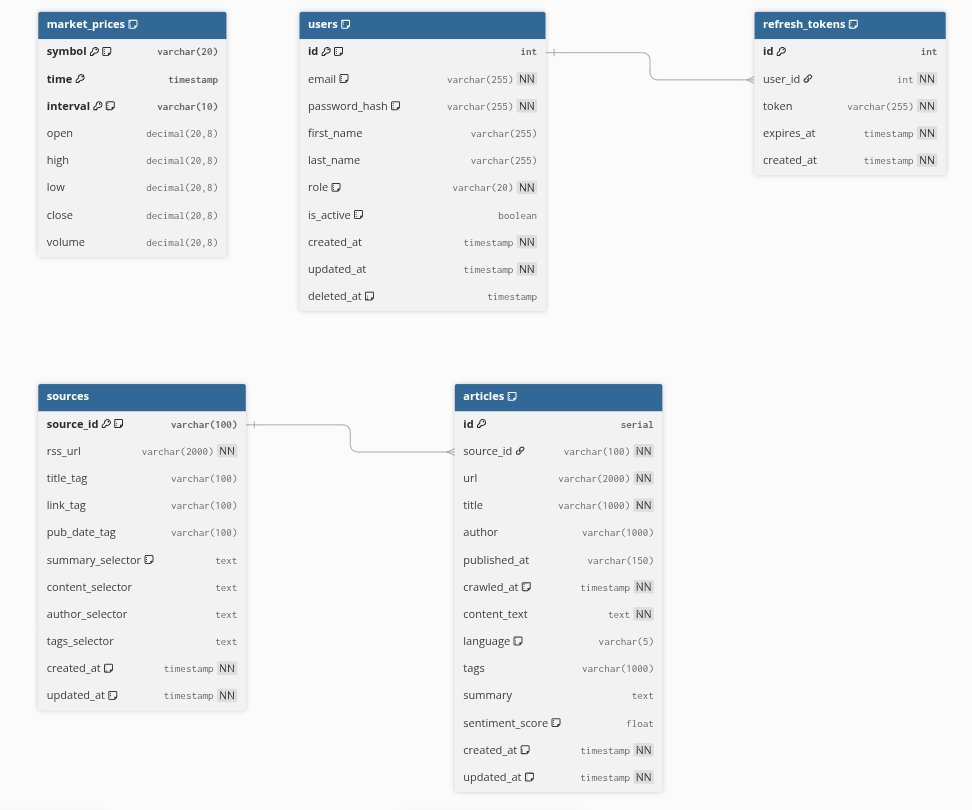
\includegraphics[width=\textwidth]{dbml.png}
\caption{Sơ đồ quan hệ cơ sở dữ liệu (DBML)}
\label{fig:dbml}
\end{figure}

\paragraph{Các bảng chính:}

\begin{itemize}
    \item \textbf{users} (Auth Service): Người dùng, phân quyền ADMIN/NORMAL/VIP.
    \item \textbf{refresh\_tokens} (Auth Service): Token làm mới phiên đăng nhập.
    \item \textbf{sources} (Crawler Service): Nguồn tin RSS (CoinDesk, CoinTelegraph, v.v.) kèm CSS selectors (Gemini AI).
    \item \textbf{articles} (Crawler Service): Bài viết crawl được, có \texttt{sentiment\_score} cập nhật bởi AI Service.
    \item \textbf{market\_prices} (Market Service): Dữ liệu nến (KLINE) từ Binance API.
\end{itemize}

\subsubsection{Mô tả chi tiết bảng}

\begin{table}[H]
\centering
\caption{Bảng users (Auth Service)}
\begin{tabular}{|l|l|l|l|}
\hline
\textbf{Cột} & \textbf{Kiểu} & \textbf{Ràng buộc} & \textbf{Mô tả} \\
\hline
id & SERIAL & PK & Primary key \\
email & VARCHAR(255) & UNIQUE, NOT NULL & Email đăng nhập \\
password\_hash & VARCHAR(255) & NOT NULL & Mật khẩu bcrypt \\
first\_name, last\_name & VARCHAR & & Tên người dùng \\
role & VARCHAR(20) & DEFAULT NORMAL & ADMIN, NORMAL, VIP \\
is\_active & BOOLEAN & DEFAULT true & Trạng thái tài khoản \\
created\_at, updated\_at & TIMESTAMP & & Thời gian \\
deleted\_at & TIMESTAMP & INDEX & Soft delete (GORM) \\
\hline
\end{tabular}
\end{table}

\begin{table}[H]
\centering
\caption{Bảng articles (Crawler Service)}
\begin{tabular}{|l|l|l|l|}
\hline
\textbf{Cột} & \textbf{Kiểu} & \textbf{Ràng buộc} & \textbf{Mô tả} \\
\hline
id & SERIAL & PK & Primary key \\
source\_id & VARCHAR(100) & FK, NOT NULL & Nguồn tin \\
url & VARCHAR(2000) & UNIQUE, NOT NULL & URL bài viết \\
title & VARCHAR(1000) & NOT NULL & Tiêu đề \\
content\_text & TEXT & NOT NULL & Nội dung \\
sentiment\_score & FLOAT & & Điểm sentiment (AI) \\
language & VARCHAR(5) & DEFAULT 'en' & en / vi \\
published\_at, crawled\_at & TIMESTAMP & & Thời gian \\
\hline
\end{tabular}
\end{table}

\begin{table}[H]
\centering
\caption{Bảng market\_prices (Market Service)}
\begin{tabular}{|l|l|l|l|}
\hline
\textbf{Cột} & \textbf{Kiểu} & \textbf{Ràng buộc} & \textbf{Mô tả} \\
\hline
symbol & VARCHAR(20) & PK & BTCUSDT, ETHUSDT, ... \\
time & TIMESTAMP & PK & Thời điểm nến đóng \\
interval & VARCHAR(10) & PK & 1m, 5m, 1h, 4h, 1d \\
open, high, low, close & DECIMAL(20,8) & & OHLC \\
volume & DECIMAL(20,8) & & Khối lượng \\
\hline
\end{tabular}
\end{table}

\subsection{Chiến lược mở rộng cơ sở dữ liệu}

Hiện tại hệ thống triển khai \textbf{single-node PostgreSQL} trong Docker Compose. Các chiến lược mở rộng sau có thể áp dụng khi scale lên production:

\subsubsection{Replication và Read Replicas}

\begin{itemize}
    \item \textbf{Đề xuất}: Triển khai PostgreSQL Streaming Replication (1 Primary + N Read Replicas).
    \item \textbf{Cách hoạt động}: Primary xử lý ghi (INSERT/UPDATE), Read Replicas phục vụ truy vấn đọc (SELECT).
    \item \textbf{Phân chia tải}: Auth Service (login/validate) và Crawler Service (list articles) có thể đọc từ replicas; Market Service (WebSocket + insert candles) ghi vào primary.
    \item \textbf{Trạng thái hiện tại}: Chưa triển khai. Cần cấu hình \texttt{wal\_level=replica}, \texttt{primary\_conninfo} trên replica.
\end{itemize}

\subsubsection{Sharding}

\begin{itemize}
    \item \textbf{Đề xuất khi scale}: Sharding theo \texttt{symbol} cho bảng \texttt{market\_prices} (time-series data lớn).
    \item \textbf{Lý do}: Mỗi cặp tiền (BTCUSDT, ETHUSDT, ...) có luồng dữ liệu độc lập; sharding giảm kích thước bảng và tăng throughput ghi.
    \item \textbf{Trạng thái hiện tại}: Chưa triển khai. Có thể dùng Citus hoặc application-level sharding.
\end{itemize}

\subsection{Kỹ thuật tối ưu hóa tại cấp độ database}

\subsubsection{Indexing}

Hệ thống đã triển khai các index sau (từ source code):

\begin{table}[H]
\centering
\caption{Các index đã triển khai}
\begin{tabular}{|l|l|l|}
\hline
\textbf{Bảng} & \textbf{Index} & \textbf{Mục đích} \\
\hline
users & idx trên email (UNIQUE) & Tra cứu đăng nhập \\
users & idx trên deleted\_at & Lọc soft-deleted \\
refresh\_tokens & idx trên user\_id & Tìm token theo user \\
refresh\_tokens & idx trên token (UNIQUE) & Validate refresh token \\
articles & idx\_articles\_source\_id & Lọc theo nguồn tin \\
articles & idx\_articles\_url (UNIQUE) & Tránh trùng lặp URL \\
articles & idx\_articles\_published\_at & Sắp xếp thời gian \\
market\_prices & idx\_market\_prices\_symbol\_time & Time-series theo symbol \\
market\_prices & idx\_market\_prices\_time & Truy vấn theo thời gian \\
\hline
\end{tabular}
\end{table}

\subsubsection{Partitioning}

\begin{itemize}
    \item \textbf{Trạng thái}: Chưa triển khai partitioning.
    \item \textbf{Đề xuất}: Bảng \texttt{market\_prices} phù hợp với \textbf{Range Partitioning} theo \texttt{time} (theo tháng hoặc theo quý) khi dữ liệu lớn. Giúp \texttt{VACUUM} và truy vấn nhanh hơn.
\end{itemize}

\subsubsection{Caching tại cấp độ database}

\begin{itemize}
    \item \textbf{Redis} (ngoài PostgreSQL): AI Service sử dụng Redis để cache kết quả prediction với key \texttt{prediction:\{symbol\}:\{horizon\}h} và TTL 5--30 phút tùy horizon.
    \item \textbf{PostgreSQL}: Sử dụng shared\_buffers mặc định. Có thể tăng \texttt{shared\_buffers} và \texttt{effective\_cache\_size} khi tối ưu production.
\end{itemize}
   % Thiết kế cơ sở dữ liệu
% =============================================================================
% KIẾN TRÚC HỆ THỐNG
% =============================================================================

\section{Kiến trúc hệ thống}
\label{sec:architecture}

Phần này mô tả kiến trúc tổng quan của hệ thống Crypto Analytics Platform dựa trên \textbf{Version 4: Microservices Event-Driven}---kiến trúc hiện đang được triển khai trong dự án.

\subsection{Sơ đồ kiến trúc tổng quan}

Hình~\ref{fig:arch-v4-overview} minh họa các thành phần chính của hệ thống và mối quan hệ giữa chúng. Luồng dữ liệu chính: Client gửi request qua API Gateway (Traefik); Gateway định tuyến đến các microservice tương ứng; các service giao tiếp bất đồng bộ qua Kafka và truy cập dữ liệu qua PostgreSQL/Redis.

\begin{figure}[H]
\centering
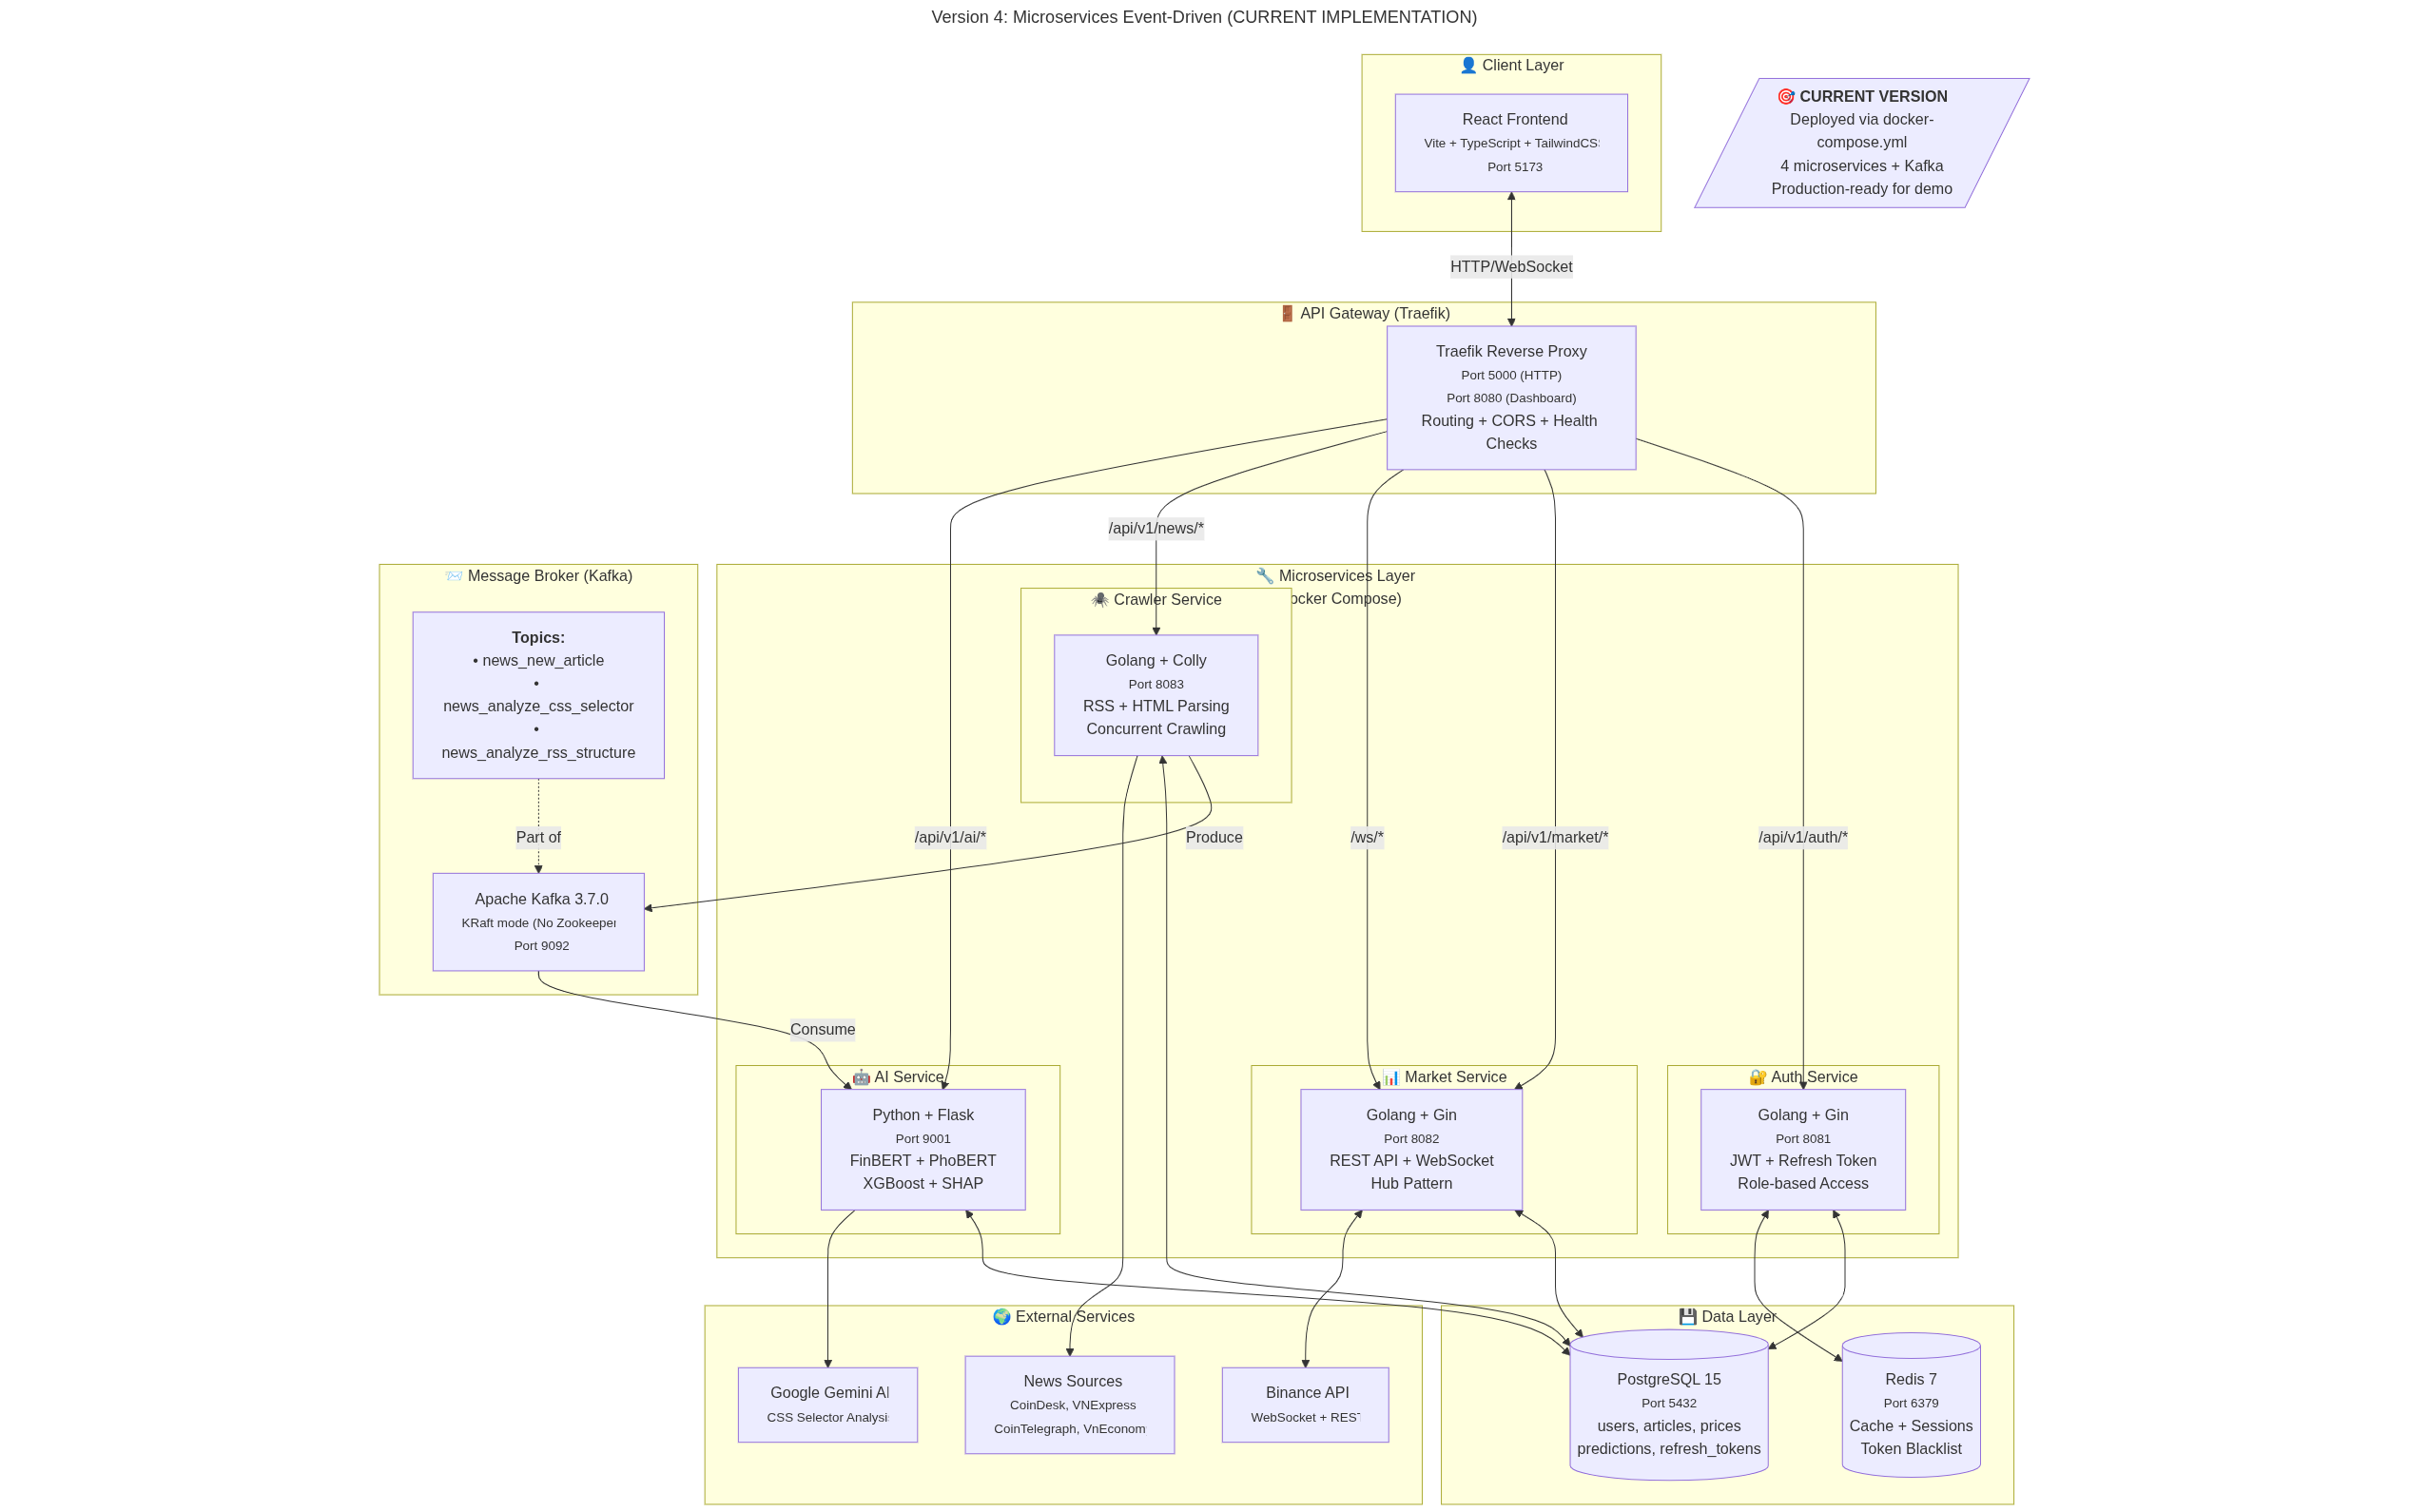
\includegraphics[width=\textwidth]{arch/ver4.png}
\caption{Kiến trúc tổng quan hệ thống (Version 4: Microservices với Kafka Event-Driven)}
\label{fig:arch-v4-overview}
\end{figure}

\subsection{Các thành phần chính và vai trò}

\subsubsection{Client (Frontend)}

\begin{itemize}
    \item \textbf{Công nghệ}: React + TypeScript, Vite; giao diện web responsive.
    \item \textbf{Vai trò}: Người dùng tương tác với hệ thống qua trình duyệt; gọi REST API để đăng nhập, lấy giá, tin tức, dự đoán AI; kết nối WebSocket để nhận dữ liệu giá realtime.
    \item \textbf{Lưu ý}: Client chỉ giao tiếp với API Gateway (HTTPS), không kết nối trực tiếp đến backend services.
\end{itemize}

\subsubsection{API Gateway (Traefik)}

\begin{itemize}
    \item \textbf{Vai trò}: Điểm vào duy nhất (single entry point) cho tất cả client requests; định tuyến theo path:
    \begin{itemize}
        \item \texttt{/api/v1/auth/*} $\to$ Auth Service (port 8081)
        \item \texttt{/api/v1/market/*} $\to$ Market Service (port 8082)
        \item \texttt{/ws/*} $\to$ Market Service WebSocket
        \item \texttt{/api/v1/news/*} $\to$ Crawler Service (port 8083)
        \item \texttt{/api/v1/ai/*} $\to$ AI Service (port 9001)
    \end{itemize}
    \item \textbf{Chức năng}: CORS handling, health checks, load balancing (khi scale nhiều instance), dashboard tại port 8080.
\end{itemize}

\subsubsection{Auth Service}

\begin{itemize}
    \item \textbf{Công nghệ}: Golang, Gin framework, GORM.
    \item \textbf{Vai trò}: Xác thực và phân quyền; đăng ký/đăng nhập với bcrypt; JWT Access Token (short-lived) + Refresh Token (long-lived, lưu DB); role-based access (NORMAL/VIP/ADMIN); token rotation và revoke.
\end{itemize}

\subsubsection{Market Service}

\begin{itemize}
    \item \textbf{Công nghệ}: Golang, WebSocket (gorilla/websocket).
    \item \textbf{Vai trò}: Kết nối Binance WebSocket API; nhận dữ liệu giá realtime; Hub pattern quản lý hàng nghìn client; topic-based subscription (theo symbol); lưu lịch sử giá vào PostgreSQL; publish updates lên Kafka.
\end{itemize}

\subsubsection{Crawler Service}

\begin{itemize}
    \item \textbf{Công nghệ}: Golang, Colly, gofeed.
    \item \textbf{Vai trò}: Thu thập tin tức từ RSS feeds (CoinDesk, CoinTelegraph, VNExpress); crawl HTML; produce Kafka messages (\texttt{news\_new\_article}, \texttt{news\_analyze\_css\_selector}) để AI Service xử lý.
\end{itemize}

\subsubsection{AI Service}

\begin{itemize}
    \item \textbf{Công nghệ}: Python, Flask, Transformers, XGBoost, SHAP.
    \item \textbf{Vai trò}: Consume Kafka từ Crawler; phân tích sentiment (FinBERT/PhoBERT); dự đoán giá (XGBoost + SHAP XAI); Gemini AI học CSS selectors.
\end{itemize}

\subsubsection{Message Broker (Apache Kafka)}

\begin{itemize}
    \item \textbf{Vai trò}: Giao tiếp bất đồng bộ giữa Crawler và AI; topics: \texttt{news\_new\_article}, \texttt{news\_analyze\_css\_selector}; cho phép replay, decoupling, và scale consumers độc lập.
\end{itemize}

\subsubsection{Database (PostgreSQL) và Cache (Redis)}

\begin{itemize}
    \item \textbf{PostgreSQL}: Cơ sở dữ liệu chính; bảng users, refresh\_tokens, sources, articles, market\_prices; shared cho các services trong implementation hiện tại.
    \item \textbf{Redis}: Cache giá hiện tại, top news; JWT blacklist; session/refresh token storage.
\end{itemize}

\subsection{Phân tích kiến trúc theo các tiêu chí}

\subsubsection{Hiệu năng (Performance)}

\begin{itemize}
    \item \textbf{WebSocket thay cho Polling}: Dữ liệu giá push-based, độ trễ thấp (hàng ms thay vì hàng giây).
    \item \textbf{Redis caching}: Giảm tải truy vấn DB cho hot data (giá, top news).
    \item \textbf{Event-driven}: Crawler và AI chạy async; AI chậm không block Crawler.
    \item \textbf{Phân tách domain}: Mỗi service tối ưu cho nhiệm vụ riêng (Golang cho I/O, Python cho AI).
\end{itemize}

\subsubsection{Khả năng mở rộng (Scalability)}

\begin{itemize}
    \item \textbf{Horizontal scaling}: Có thể scale từng service độc lập (vd. \texttt{docker-compose up -d --scale market-service=3}).
    \item \textbf{Topic-based WebSocket Hub}: Hỗ trợ nhiều client đồng thời; có thể mở rộng qua Kafka hoặc Redis Pub/Sub khi nhiều Market instances.
    \item \textbf{Kafka consumers}: Thêm consumer cho AI Service để tăng throughput xử lý tin tức.
\end{itemize}

\subsubsection{Độ tin cậy (Reliability)}

\begin{itemize}
    \item \textbf{Fault isolation}: AI Service crash không ảnh hưởng Market/Auth; Market Service vẫn phục vụ WebSocket khi Kafka tạm lỗi (graceful degradation).
    \item \textbf{Auto-reconnect}: Market Service kết nối lại Binance với exponential backoff khi mất kết nối.
    \item \textbf{Kafka replay}: Có thể replay messages nếu AI Service fail.
\end{itemize}

\subsubsection{Bảo mật (Security)}

\begin{itemize}
    \item \textbf{API Gateway}: Single entry point; kiểm tra CORS; có thể thêm rate limiting.
    \item \textbf{JWT + Refresh Token}: Access token ngắn hạn; Refresh token lưu DB, có thể revoke; rotation mỗi lần refresh.
    \item \textbf{Phân quyền}: Role-based (NORMAL/VIP/ADMIN); VIP required cho API AI.
    \item \textbf{Zero-Trust}: Mọi request phải authenticate; validate input; có thể mở rộng mTLS giữa services (Service Mesh).
\end{itemize}
 % Kiến trúc hệ thống (Version 4)
% =============================================================================
% CHAPTER: SCALING ARCHITECTURE - QUÁ TRÌNH SCALE-UP HỆ THỐNG
% =============================================================================

\chapter{Quá trình Scale-up Kiến trúc Hệ thống}

\section{Tổng quan về Scaling}

Trong quá trình phát triển hệ thống Crypto Analytics Platform, kiến trúc được thiết kế theo nguyên tắc \textbf{progressive scaling} - bắt đầu từ đơn giản và mở rộng dần theo nhu cầu thực tế. Chương này trình bày 5 phiên bản kiến trúc tương ứng với các giai đoạn phát triển khác nhau.

\begin{table}[H]
\centering
\caption{Tổng quan các phiên bản kiến trúc}
\begin{tabular}{|c|l|c|l|}
\hline
\textbf{Version} & \textbf{Tên gọi} & \textbf{Users} & \textbf{Đặc điểm chính} \\
\hline
V1 & Single Box Monolith & 10-100 & Tất cả trong 1 server \\
\hline
V2 & Users+ & 100-1,000 & Tách Database + Object Storage \\
\hline
V3 & Users++ & 1,000-10,000 & Load Balancer + Scale ngang \\
\hline
V4 & Users+++ & 10,000-100,000 & Microservices + API Gateway \\
\hline
V5 & Users++++ & 100,000-1M+ & Autoscaling + Data Lake \\
\hline
\end{tabular}
\end{table}

% =============================================================================
\section{Version 1: Single Box Monolith}
% =============================================================================

\subsection{Bối cảnh và Giả định}

\begin{itemize}
    \item \textbf{Số lượng user}: Vài chục đến vài trăm người dùng
    \item \textbf{Mục tiêu}: Chạy demo ổn định, chưa cần high availability
    \item \textbf{Độ trễ}: Chấp nhận được ở mức cơ bản
    \item \textbf{Phù hợp}: Giai đoạn phát triển đồ án, MVP, Proof of Concept
\end{itemize}

\subsection{Thành phần Kiến trúc}

Toàn bộ hệ thống chạy trên \textbf{1 EC2 instance} (hoặc 1 VPS) duy nhất trong VPC:

\subsubsection{Web Server + Ứng dụng Monolith}

\begin{itemize}
    \item \textbf{REST API + WebSocket Server}:
    \begin{itemize}
        \item Lấy giá từ Binance API (REST) để build lịch sử
        \item Mở WebSocket đến Binance để nhận giá realtime và forward ra cho client
    \end{itemize}
    
    \item \textbf{Crawler tin tức}:
    \begin{itemize}
        \item Cron job/Background task (Celery/RQ hoặc đơn giản là cron + script)
        \item Gọi HTTP đến nhiều trang báo, parse HTML
        \item Trích xuất: Tiêu đề, timestamp, nguồn, link, nội dung, sentiment
        \item Lưu raw HTML + thông tin đã trích xuất
    \end{itemize}
    
    \item \textbf{Service AI}:
    \begin{itemize}
        \item Gọi model AI từ local (file .pt, .h5) hoặc API ngoài
        \item Align tin tức với giá lịch sử để tạo feature
    \end{itemize}
    
    \item \textbf{Module Account}:
    \begin{itemize}
        \item Đăng ký/Đăng nhập
        \item Profile user, watchlist cặp tiền
        \item Lưu config GUI (layout chart, khung thời gian yêu thích)
    \end{itemize}
\end{itemize}

\subsubsection{Database và Storage}

\begin{itemize}
    \item \textbf{PostgreSQL/MySQL} cài trên cùng máy:
    \begin{itemize}
        \item Bảng: users, news, prices, signals, logs
    \end{itemize}
    \item \textbf{Local Disk Storage}:
    \begin{itemize}
        \item Raw HTML, file model AI, logs
    \end{itemize}
\end{itemize}

\subsection{Phân tích Trade-offs}

\begin{table}[H]
\centering
\caption{Trade-offs Version 1}
\begin{tabular}{|p{6cm}|p{6cm}|}
\hline
\textbf{Ưu điểm} & \textbf{Nhược điểm} \\
\hline
Đơn giản, dễ code, dễ deploy & Không scale ngang được \\
\hline
Chi phí thấp (1 server) & Single point of failure \\
\hline
Debug nhanh, ít network hop & Tất cả modules cạnh tranh tài nguyên \\
\hline
Phù hợp giai đoạn đồ án đầu & Chỉ scale dọc (CPU/RAM/disk) \\
\hline
\end{tabular}
\end{table}

% =============================================================================
\section{Version 2: Users+ - Tách Database + Object Storage}
% =============================================================================

\subsection{Trigger để Scale}

Khi số lượng user tăng (vài ngàn), crawler lấy tin từ nhiều nguồn hơn, dữ liệu tin tức và giá lịch sử tăng rất nhanh, cần tách database và storage ra khỏi application server.

\subsection{Thay đổi Kiến trúc}

\begin{itemize}
    \item \textbf{EC2 App Server}: Chạy monolith như cũ, nhưng bỏ DB ra ngoài
    \begin{itemize}
        \item Web + API + WebSocket + Crawler + AI (vẫn là 1 codebase)
    \end{itemize}
    
    \item \textbf{RDS (Managed Database)}:
    \begin{itemize}
        \item Tách DB ra thành máy riêng (managed service)
        \item Bảng tin tức, giá, user, signals
        \item Có thể scale riêng (tăng RAM, IOPS)
    \end{itemize}
    
    \item \textbf{S3 (Object Storage)}:
    \begin{itemize}
        \item Raw HTML của news (để re-parse khi site đổi HTML)
        \item File model AI
        \item Log lớn, file backup
    \end{itemize}
    
    \item \textbf{VPC Configuration}:
    \begin{itemize}
        \item App server ở public subnet
        \item RDS + S3 access ở private (qua endpoint, security group)
    \end{itemize}
    
    \item \textbf{Security}:
    \begin{itemize}
        \item Security group chỉ cho App server connect đến RDS
        \item Port mở ra internet: 80/443
    \end{itemize}
\end{itemize}

\subsection{Lợi ích của Version 2}

\begin{itemize}
    \item DB có thể scale riêng (tăng RAM, IOPS)
    \item S3 xử lý tốt khối lượng lớn file tin tức \& raw HTML (1 TB/tháng là bình thường)
    \item Ứng dụng nhẹ hơn, không lo full disk vì news/history
    \item \textbf{Hạn chế}: Vẫn chỉ có 1 app server → dễ nghẽn khi WebSocket connection nhiều
\end{itemize}

% =============================================================================
\section{Version 3: Users++ - Load Balancer + Scale ngang}
% =============================================================================

\subsection{Trigger để Scale}

\begin{itemize}
    \item Hàng chục nghìn user
    \item Biểu đồ realtime cho nhiều cặp tiền, đa khung thời gian
    \item Crawler tin từ nhiều site, AI phân tích nặng hơn
\end{itemize}

\subsection{Thay đổi Kiến trúc}

\subsubsection{Application Load Balancer (ALB)}
\begin{itemize}
    \item Nhận HTTP/HTTPS + WebSocket từ client
    \item Phân phối request đến nhiều App server
    \item Pattern: "Horizontal scaling web servers" trong Scaling AWS
\end{itemize}

\subsubsection{App Server Auto Scaling Group}
Nhiều EC2 instance chạy:
\begin{itemize}
    \item API cho GUI (lấy news đã xử lý, giá, signal)
    \item WebSocket để push giá realtime \& tín hiệu AI
    \item Render chart (TradingView-like)
    \item \textbf{Không} chạy crawler \& jobs nặng AI (để tránh block)
\end{itemize}

\subsubsection{Worker Cluster (Crawler + AI)}
Một Auto Scaling Group khác với role "Worker":
\begin{itemize}
    \item \textbf{Crawler Service}:
    \begin{itemize}
        \item Gửi HTTP đến các site news
        \item Rule-based theo CSS selector/XPath cho từng site
        \item ML model phân loại block (title, body, author)
        \item Đẩy kết quả vào DB + lưu raw HTML lên S3
    \end{itemize}
    \item \textbf{AI Service}:
    \begin{itemize}
        \item Consumes news + price history
        \item Gọi model AI để tạo sentiment, dự đoán xu hướng
        \item Lưu signals vào DB
    \end{itemize}
\end{itemize}

\subsubsection{Message Queue (SQS/Kafka)}
\begin{itemize}
    \item \textbf{News Fetch Queue}: app tạo job khi cần crawl nguồn mới
    \item \textbf{AI Analysis Queue}: crawler xong → đẩy job để AI xử lý
    \item Pattern: "Queues + Workers" trong Asynchronism
\end{itemize}

\subsubsection{RDS với Read Replicas}
\begin{itemize}
    \item Master: ghi
    \item 1-2 read replica: phục vụ query đọc nặng (news list, history chart)
\end{itemize}

\subsubsection{Cache Layer (Redis/ElastiCache)}
Cache-aside pattern cho:
\begin{itemize}
    \item Giá hiện tại của BTCUSDT, ETHUSDT, ...
    \item Top news mới nhất
    \item Tín hiệu AI nóng
\end{itemize}

\subsection{Lý do cần Version 3}

\begin{itemize}
    \item Nhu cầu người dùng tăng: xem đa cặp tiền, đa khung thời gian, realtime
    \item Hàng ngàn WebSocket connection → cần nhiều app server
    \item Công việc nặng (crawler, AI) tách ra để không làm web bị lag
    \item Queue + Worker giúp xử lý bất đồng bộ, có khả năng backpressure
    \item ALB + nhiều instance + read replica DB → high availability
\end{itemize}

% =============================================================================
\section{Version 4: Users+++ - Microservices + API Gateway}
% =============================================================================

\subsection{Trigger để Scale}

\begin{itemize}
    \item Lên tới trăm nghìn user
    \item Yêu cầu tính modular để đội dev chia nhau làm
    \item Cần tăng độ tin cậy từng module và scale độc lập
\end{itemize}

\subsection{Kiến trúc Microservices}

\subsubsection{API Gateway (Nginx/Kong/Envoy)}
Entry point duy nhất cho client:
\begin{itemize}
    \item \texttt{/news/*} → News Service
    \item \texttt{/prices/*} → Market Data Service
    \item \texttt{/ai/*} → AI Service
    \item \texttt{/account/*} → Account Service
\end{itemize}

Thực hiện:
\begin{itemize}
    \item AuthN/AuthZ (JWT, OAuth)
    \item Rate limiting, request logging
\end{itemize}

\subsubsection{Market Data Service}
\begin{itemize}
    \item Kết nối WebSocket đến Binance, duy trì stream giá realtime
    \item Lưu giá lịch sử vào Time-series DB hoặc RDS riêng
    \item Expose:
    \begin{itemize}
        \item REST: lịch sử giá, multi-timeframe (1m, 5m, 1h, 1d)
        \item WebSocket/SSE: giá hiện tại \& candlestick realtime
    \end{itemize}
\end{itemize}

\subsubsection{News Service}
\begin{itemize}
    \item Quản lý crawler worker
    \item Lưu, index tin tức trong DB riêng
    \item Elasticsearch/OpenSearch để search nhanh
\end{itemize}

\subsubsection{AI Service}
\begin{itemize}
    \item Nhận tin tức đã align với giá
    \item Trả về: Sentiment score, Prediction (UP/DOWN), Explanation
    \item Wrap model hộp đen (HuggingFace, SageMaker endpoint)
\end{itemize}

\subsubsection{Account Service}
\begin{itemize}
    \item User, auth, profile, watchlist, setting GUI
    \item Token-based auth (JWT) để các service khác verify
\end{itemize}

\subsubsection{Message Bus (Kafka/Kinesis)}
Topics:
\begin{itemize}
    \item \texttt{news\_raw}: Raw news data từ crawler
    \item \texttt{news\_parsed}: Parsed news sau processing
    \item \texttt{price\_ticks}: Real-time price updates
    \item \texttt{ai\_signals}: AI prediction signals
\end{itemize}

\subsection{Lý do chuyển sang Microservices}

\begin{table}[H]
\centering
\caption{Lợi ích của Microservices Architecture}
\begin{tabular}{|l|p{8cm}|}
\hline
\textbf{Khía cạnh} & \textbf{Lợi ích} \\
\hline
Domain rõ ràng & 4 phần tách biệt (news, price, AI, account) phù hợp chia service \\
\hline
Scale độc lập & Market Data cần CPU/network, AI cần GPU, News cần IO \\
\hline
Độ tin cậy & AI Service lỗi, chart + news vẫn chạy (graceful degradation) \\
\hline
Team phát triển & Mỗi team phụ trách 1 service, độc lập deploy \\
\hline
\end{tabular}
\end{table}

% =============================================================================
\section{Version 5: Users++++ - Autoscaling + Data Lake}
% =============================================================================

\subsection{Trigger để Scale}

\begin{itemize}
    \item Hàng triệu user
    \item Khối lượng tin tức \& giá rất lớn (1B writes/tháng, 100B reads/tháng)
    \item Yêu cầu AI nâng cao với causal inference
\end{itemize}

\subsection{Thành phần Bổ sung}

\subsubsection{Autoscaling cho từng nhóm}
Auto Scaling Group cho:
\begin{itemize}
    \item Market Data Service
    \item News Service
    \item AI Service
    \item Account/GUI Service
\end{itemize}

Scale metrics:
\begin{itemize}
    \item CPU utilization
    \item Number of connections
    \item Message queue lag
    \item Custom business metrics
\end{itemize}

\subsubsection{Global CDN}
\begin{itemize}
    \item Frontend static (JS/CSS, bundle TradingView-like) qua CloudFront
    \item Giảm tải App server, giảm latency cho user toàn cầu
\end{itemize}

\subsubsection{Data Warehouse / Data Lake}
Đổ news + price + signals về:
\begin{itemize}
    \item Redshift / BigQuery / Snowflake hoặc S3-based data lake
    \item Training model mới
    \item Phân tích offline (backtest, AB test chiến lược)
\end{itemize}

\subsubsection{Feature Store cho AI}
\begin{itemize}
    \item Lưu các feature đã xử lý (sentiment series, lag features, volume, volatility)
    \item Giúp inference nhanh, training reproducible
\end{itemize}

\subsubsection{Observability / Monitoring}
\begin{itemize}
    \item \textbf{Metrics}: Latency API, error rate, throughput, queue lag, DB load
    \item \textbf{Logs}: Centralized log (ELK, CloudWatch Logs, Splunk)
    \item \textbf{Alerts}: PagerDuty/Email khi lỗi 5xx tăng, latency tăng, AI timeout
\end{itemize}

\subsection{Lý do cần Version 5}

\begin{itemize}
    \item \textbf{Scale chi tiết theo từng tải}:
    \begin{itemize}
        \item Giờ cao điểm (US business hours) giá/WS load tăng → autoscale Market Data
        \item Major news (SEC, ETF, regulation) → autoscale News + AI Worker
    \end{itemize}
    \item \textbf{High Availability}:
    \begin{itemize}
        \item Multiple AZs, autoscaling, health check
        \item Rollback, canary deployment
    \end{itemize}
    \item \textbf{AI nâng cao}:
    \begin{itemize}
        \item Cần nhiều dữ liệu lịch sử để làm causal inference
        \item Data lake \& warehouse phục vụ training model
    \end{itemize}
\end{itemize}

% =============================================================================
\section{So sánh Tổng quan các Phiên bản}
% =============================================================================

\begin{table}[H]
\centering
\caption{So sánh chi tiết các phiên bản kiến trúc}
\resizebox{\textwidth}{!}{
\begin{tabular}{|l|c|c|c|c|c|}
\hline
\textbf{Đặc điểm} & \textbf{V1} & \textbf{V2} & \textbf{V3} & \textbf{V4} & \textbf{V5} \\
\hline
Số lượng user & 10-100 & 100-1K & 1K-10K & 10K-100K & 100K-1M+ \\
\hline
App Servers & 1 & 1 & N (ASG) & N per service & N per service \\
\hline
Database & Local & RDS & RDS + Replicas & Per-service DB & Multi-AZ + Lake \\
\hline
Load Balancer & None & None & ALB & API Gateway & API Gateway \\
\hline
Message Queue & None & None & SQS/Kafka & Kafka & Kafka Cluster \\
\hline
Cache & None & None & Redis & Redis & Redis Cluster \\
\hline
Storage & Local & S3 & S3 & S3 & S3 + Data Lake \\
\hline
Monitoring & Basic & Basic & CloudWatch & Prometheus & Full Stack \\
\hline
Availability & Low & Medium & High & High & Very High \\
\hline
Complexity & Low & Low & Medium & High & Very High \\
\hline
Cost & \$ & \$\$ & \$\$\$ & \$\$\$\$ & \$\$\$\$\$ \\
\hline
\end{tabular}
}
\end{table}

% =============================================================================
\section{Kết luận}
% =============================================================================

Quá trình scale-up kiến trúc của Crypto Analytics Platform tuân theo nguyên tắc:

\begin{enumerate}
    \item \textbf{Start Simple}: Bắt đầu với monolith đơn giản, tập trung vào business logic
    \item \textbf{Measure First}: Đo đạc bottleneck trước khi tối ưu
    \item \textbf{Scale Incrementally}: Tách từng phần khi cần thiết, không over-engineer
    \item \textbf{Embrace Trade-offs}: Mỗi quyết định kiến trúc đều có trade-off về complexity vs scalability
\end{enumerate}

Dự án hiện tại đang ở \textbf{Version 4} với kiến trúc microservices, sử dụng:
\begin{itemize}
    \item 4 services: Auth, Market, Crawler, AI
    \item Kafka message broker
    \item PostgreSQL + Redis
    \item Docker Compose cho orchestration
\end{itemize}

Kiến trúc này phù hợp với quy mô đồ án và có thể dễ dàng mở rộng lên Version 5 khi cần thiết.
    % Quá trình scale-up kiến trúc hệ thống
% =============================================================================
% ÁP DỤNG DESIGN PATTERNS
% =============================================================================

\section{Áp dụng Design Patterns}
\label{sec:design-patterns}

Hệ thống Crypto Analytics Platform áp dụng nhiều mẫu Design Patterns quan trọng, giúp mã nguồn dễ bảo trì, mở rộng và tái sử dụng. Phần này xác định các pattern đã triển khai, giải thích ý nghĩa, lợi ích và minh họa bằng sơ đồ Mermaid (mã nguồn trong \texttt{mermaid/}).

\subsection{Singleton / Single Instance}

\subsubsection{Mô tả}

\textbf{Intent}: Đảm bảo class chỉ có một instance và cung cấp điểm truy cập toàn cục.

\subsubsection{Áp dụng trong hệ thống}

\begin{enumerate}
    \item \textbf{WebSocket Hub} (\texttt{market-service/pkg/websocket/hub.go}): Một instance Hub duy nhất quản lý tất cả WebSocket clients và topic subscriptions. Tất cả connections đều gửi/nhận qua cùng một Hub.
    
    \item \textbf{Redis Cache} (\texttt{ai-service-python/internal/cache/redis\_cache.py}): Module-level instance \texttt{cache = RedisCache()} được import và dùng chung toàn AI Service cho prediction cache.
\end{enumerate}

\subsubsection{Lợi ích}

\begin{itemize}
    \item \textbf{WebSocket Hub}: Tránh phân mảnh kết nối, quản lý tập trung subscriptions, dễ broadcast theo topic.
    \item \textbf{Redis Cache}: Một kết nối Redis dùng chung, tiết kiệm tài nguyên, đảm bảo cache nhất quán.
\end{itemize}

\subsubsection{Sơ đồ minh họa}

\begin{figure}[H]
\centering
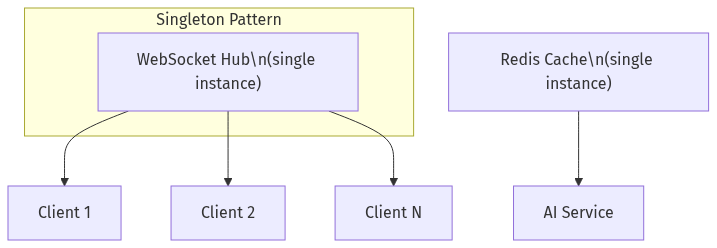
\includegraphics[width=0.7\textwidth]{pattern_singleton}
\caption{Singleton Pattern: WebSocket Hub và Redis Cache}
\label{fig:pattern-singleton}
\end{figure}

\subsection{Adapter Pattern}

\subsubsection{Mô tả}

\textbf{Intent}: Cho phép objects có interface không tương thích làm việc cùng nhau thông qua lớp wrapper.

\subsubsection{Áp dụng trong hệ thống}

\textbf{Binance Client} (\texttt{market-service/pkg/binance/client.go}): Binance API trả về mảng \texttt{[][]interface{}} cho Klines; hệ thống cần \texttt{[]*model.MarketPrice}. Hàm \texttt{parseKline()} đóng vai trò Adapter chuyển đổi format Binance sang format nội bộ.

\subsubsection{Lợi ích}

\begin{itemize}
    \item Tách biệt logic xử lý API bên ngoài khỏi domain model.
    \item Dễ thay thế hoặc thêm nguồn dữ liệu khác (CoinGecko, Kraken) mà không thay đổi core logic.
\end{itemize}

\subsubsection{Sơ đồ minh họa}

\begin{figure}[H]
\centering
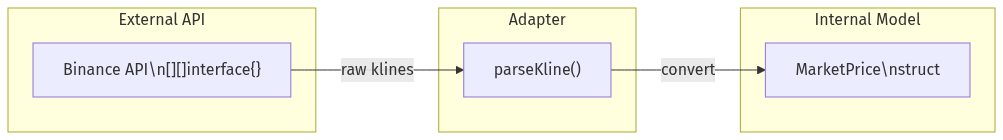
\includegraphics[width=0.9\textwidth]{pattern_adapter}
\caption{Adapter Pattern: Binance API $\rightarrow$ MarketPrice}
\label{fig:pattern-adapter}
\end{figure}

\subsection{Observer Pattern (Pub/Sub)}

\subsubsection{Mô tả}

\textbf{Intent}: Định nghĩa quan hệ one-to-many: khi object chủ thay đổi, tất cả observers được thông báo.

\subsubsection{Áp dụng trong hệ thống}

\textbf{Topic-based WebSocket Hub}: Clients subscribe vào topics (e.g., \texttt{btcusdt@kline\_1m}); khi có dữ liệu mới từ Binance WebSocket, Hub broadcast đến tất cả clients đã subscribe topic đó. Clients là observers, Hub là subject.

\subsubsection{Lợi ích}

\begin{itemize}
    \item Loose coupling: Clients không cần biết nguồn dữ liệu.
    \item Dễ scale: Thêm clients mới chỉ cần subscribe topic tương ứng.
\end{itemize}

\subsubsection{Sơ đồ minh họa}

\begin{figure}[H]
\centering
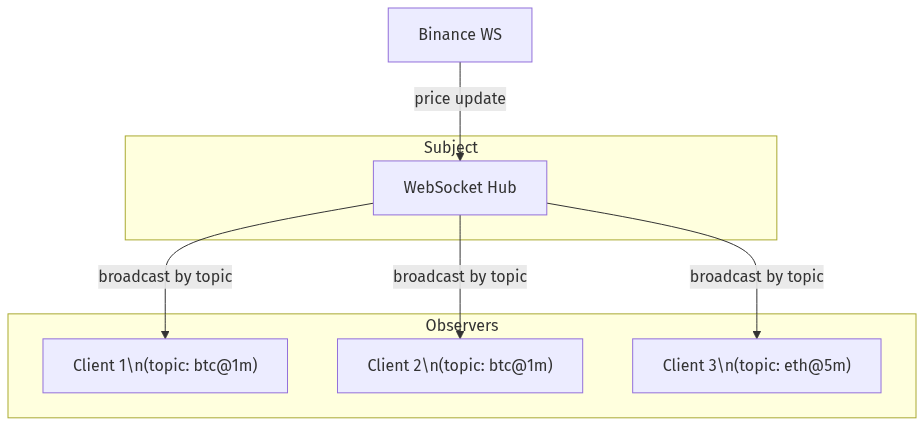
\includegraphics[width=0.8\textwidth]{pattern_observer}
\caption{Observer Pattern: Topic-based WebSocket Hub}
\label{fig:pattern-observer}
\end{figure}

\subsection{Strategy Pattern (implicit)}

\subsubsection{Mô tả}

\textbf{Intent}: Định nghĩa họ thuật toán, đóng gói từng thuật toán và cho phép thay thế linh hoạt.

\subsubsection{Áp dụng trong hệ thống}

\textbf{Sentiment Analysis} (\texttt{ai-service-python/internal/sentiment/sentiment.py}): Hai chiến lược khác nhau --- FinBERT cho tiếng Anh, PhoBERT cho tiếng Việt. Pipeline tự động chọn model dựa trên \texttt{language} của bài viết.

\subsubsection{Lợi ích}

\begin{itemize}
    \item Dễ thêm ngôn ngữ mới (chỉ cần thêm strategy mới).
    \item Logic chọn model tập trung, dễ test.
\end{itemize}

\subsubsection{Sơ đồ minh họa}

\begin{figure}[H]
\centering
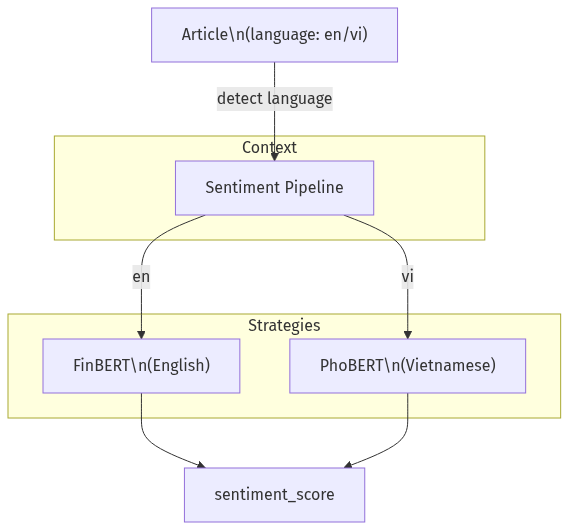
\includegraphics[width=0.7\textwidth]{pattern_strategy}
\caption{Strategy Pattern: Sentiment (FinBERT / PhoBERT)}
\label{fig:pattern-strategy}
\end{figure}

\subsection{Template Method (implicit)}

\subsubsection{Mô tả}

\textbf{Intent}: Định nghĩa skeleton của thuật toán trong superclass, subclass override các bước cụ thể.

\subsubsection{Áp dụng trong hệ thống}

\textbf{Prediction Pipeline} (\texttt{ai-service-python/internal/prediction.py}): Pipeline cố định: \texttt{load\_price\_data()} $\rightarrow$ \texttt{load\_news\_data()} $\rightarrow$ \texttt{process\_news()} (align với price buckets) $\rightarrow$ \texttt{create\_price\_features()} $\rightarrow$ \texttt{train()}/\texttt{predict()}. Các bước cụ thể có thể điều chỉnh (features, horizons) nhưng luồng tổng thể không đổi.

\subsubsection{Lợi ích}

\begin{itemize}
    \item Đảm bảo thứ tự xử lý đúng (news alignment, feature engineering).
    \item Tái sử dụng logic chung, tránh lặp code.
\end{itemize}

\subsubsection{Sơ đồ minh họa}

\begin{figure}[H]
\centering
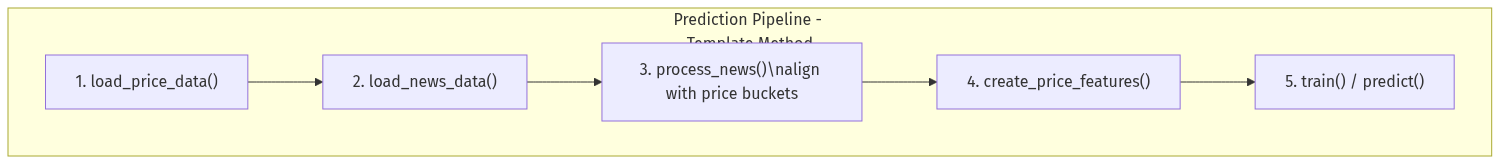
\includegraphics[width=0.75\textwidth]{pattern_template_method}
\caption{Template Method: Prediction Pipeline}
\label{fig:pattern-template}
\end{figure}

\subsection{Tổng kết Design Patterns}

\begin{table}[H]
\centering
\caption{Các Design Patterns đã áp dụng}
\begin{tabular}{|l|l|l|}
\hline
\textbf{Pattern} & \textbf{Vị trí} & \textbf{Mục đích} \\
\hline
Singleton & WebSocket Hub, Redis Cache & Single instance, shared state \\
\hline
Adapter & Binance Client parseKline & Chuyển đổi API format \\
\hline
Observer & Topic-based WebSocket & Pub/Sub real-time \\
\hline
Strategy & Sentiment (FinBERT/PhoBERT) & Chọn model theo ngôn ngữ \\
\hline
Template Method & Prediction Pipeline & Luồng xử lý cố định \\
\hline
\end{tabular}
\end{table}
 % Áp dụng Design Patterns
% =============================================================================
% PHẦN ỨNG DỤNG
% =============================================================================

\section{Phần ứng dụng}
\label{sec:ung-dung}

Phần này mô tả các tính năng đã triển khai và các giao diện màn hình (GUI) quan trọng trong đồ án Crypto Analytics Platform.

\subsection{Các tính năng đã thực hiện}

\subsubsection{1. Xác thực và phân quyền}

\begin{itemize}
    \item \textbf{Đăng ký / Đăng nhập}: Người dùng đăng ký bằng email và mật khẩu; đăng nhập nhận JWT access token và refresh token.
    \item \textbf{Phân quyền}: Ba vai trò --- \texttt{NORMAL} (Free), \texttt{VIP}, \texttt{ADMIN}. Tài khoản VIP/ADMIN mới truy cập được AI Prediction Panel.
    \item \textbf{Protected Routes}: Frontend kiểm tra role trước khi hiển thị tính năng; Backend middleware \texttt{RequireVIP} bảo vệ API AI.
\end{itemize}

\subsubsection{2. Biểu đồ giá thời gian thực (TradingView-like)}

\begin{itemize}
    \item \textbf{Đa cặp tiền}: Chọn symbol (BTCUSDT, ETHUSDT, BNBUSDT, SOLUSDT, v.v.) qua dropdown.
    \item \textbf{Đa khung thời gian}: Mỗi ô biểu đồ có timeframe riêng (1m, 5m, 15m, 1h, 4h, 1d).
    \item \textbf{Real-time}: WebSocket nhận cập nhật giá mới từ Binance; biểu đồ nến cập nhật ngay khi có dữ liệu.
    \item \textbf{Lightweight Charts}: Sử dụng thư viện TradingView Lightweight Charts cho giao diện chuyên nghiệp.
\end{itemize}

\subsubsection{3. Tin tức tài chính (News Crawler)}

\begin{itemize}
    \item \textbf{Danh sách tin}: Lấy bài viết từ nhiều nguồn (CoinDesk, CoinTelegraph, v.v.) qua RSS; hiển thị theo thời gian với pagination dạng cursor.
    \item \textbf{Lọc theo nguồn và ngôn ngữ}: Filter theo \texttt{source\_id}, \texttt{language} (en/vi).
    \item \textbf{Sentiment score}: Mỗi bài có điểm sentiment (cập nhật bởi AI Service); hiển thị trên danh sách khi có.
\end{itemize}

\subsubsection{4. AI Prediction (VIP/ADMIN)}

\begin{itemize}
    \item \textbf{Dự đoán xu hướng}: Chọn symbol và prediction horizon (1h, 4h, 24h); gọi API AI Service trả về hướng UP/DOWN và confidence.
    \item \textbf{SHAP Feature Importance}: Hiển thị đóng góp của từng feature (technical indicators, sentiment) vào kết quả dự đoán.
    \item \textbf{Top News}: Các bài tin có ảnh hưởng lớn nhất kèm keywords.
    \item \textbf{Train model}: Admin có thể gọi API train lại model với symbol/horizon/years tùy chọn.
\end{itemize}

\subsubsection{5. Quản lý nguồn tin (Admin)}

\begin{itemize}
    \item \textbf{CRUD Sources}: Thêm/sửa/xóa nguồn RSS; cấu hình RSS URL và các tag (title, link, pubDate).
    \item \textbf{Gemini AI Analyze}: Gửi mẫu HTML lên AI Service; Gemini trả về CSS selectors cho content, author, summary; lưu vào database.
\end{itemize}

\subsubsection{6. Quản lý người dùng (Admin)}

\begin{itemize}
    \item \textbf{Danh sách users}: Bảng hiển thị tên, email, role (ADMIN, VIP, NORMAL).
    \item \textbf{Đổi role}: Admin có thể thay đổi role của user khác (trừ chính mình).
    \item \textbf{Bảo vệ Admin}: Tài khoản Admin hiện tại không thể thay đổi role; hiển thị \textit{Protected}.
\end{itemize}

\subsection{Giao diện màn hình quan trọng}

\subsubsection{Dashboard}

Màn hình chính sau khi đăng nhập (Hình~\ref{fig:gui-dashboard}):
\begin{itemize}
    \item \textbf{Layout}: Grid 4 cột biểu đồ (2x2) + 1 cột bên phải cho AI Prediction (nếu VIP/ADMIN).
    \item \textbf{Symbol Selector}: Dropdown chọn cặp tiền ở header; áp dụng cho tất cả biểu đồ và panel prediction.
    \item \textbf{Chart Containers}: Mỗi ô hiển thị biểu đồ nến cho symbol đã chọn, với timeframe riêng (1m, 5m, 15m, 1h).
    \item \textbf{Prediction Panel}: Cho VIP/ADMIN --- chọn horizon, gọi API prediction, hiển thị kết quả dự đoán, SHAP, top news. Tài khoản Free thấy thông báo yêu cầu nâng cấp VIP.
\end{itemize}

\begin{figure}[H]
\centering
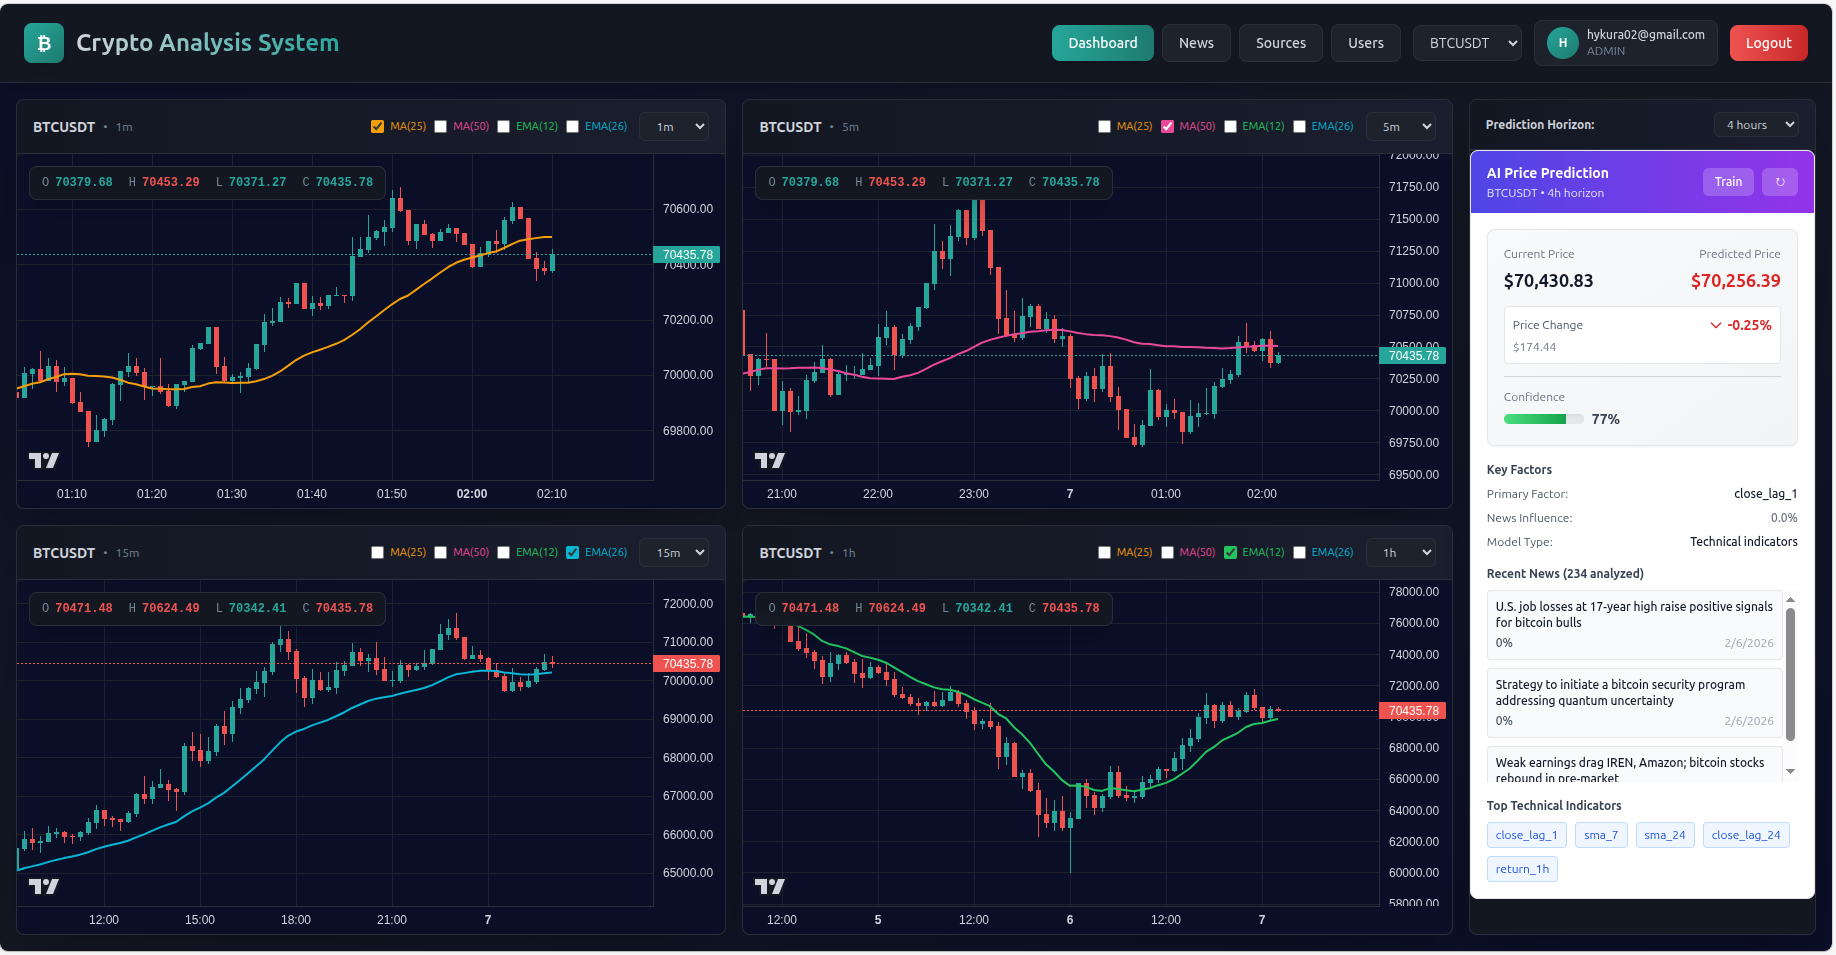
\includegraphics[width=\textwidth]{gui_dashboard}
\caption{Giao diện Dashboard: biểu đồ giá thời gian thực và AI Prediction Panel}
\label{fig:gui-dashboard}
\end{figure}

\subsubsection{News}

\begin{itemize}
    \item \textbf{Danh sách bài viết}: Dạng card/list với tiêu đề, tóm tắt, nguồn, thời gian, sentiment (nếu có).
    \item \textbf{Sidebar}: Tin tức mới nhất; có thể tích hợp vào Dashboard.
\end{itemize}

\begin{figure}[H]
\centering
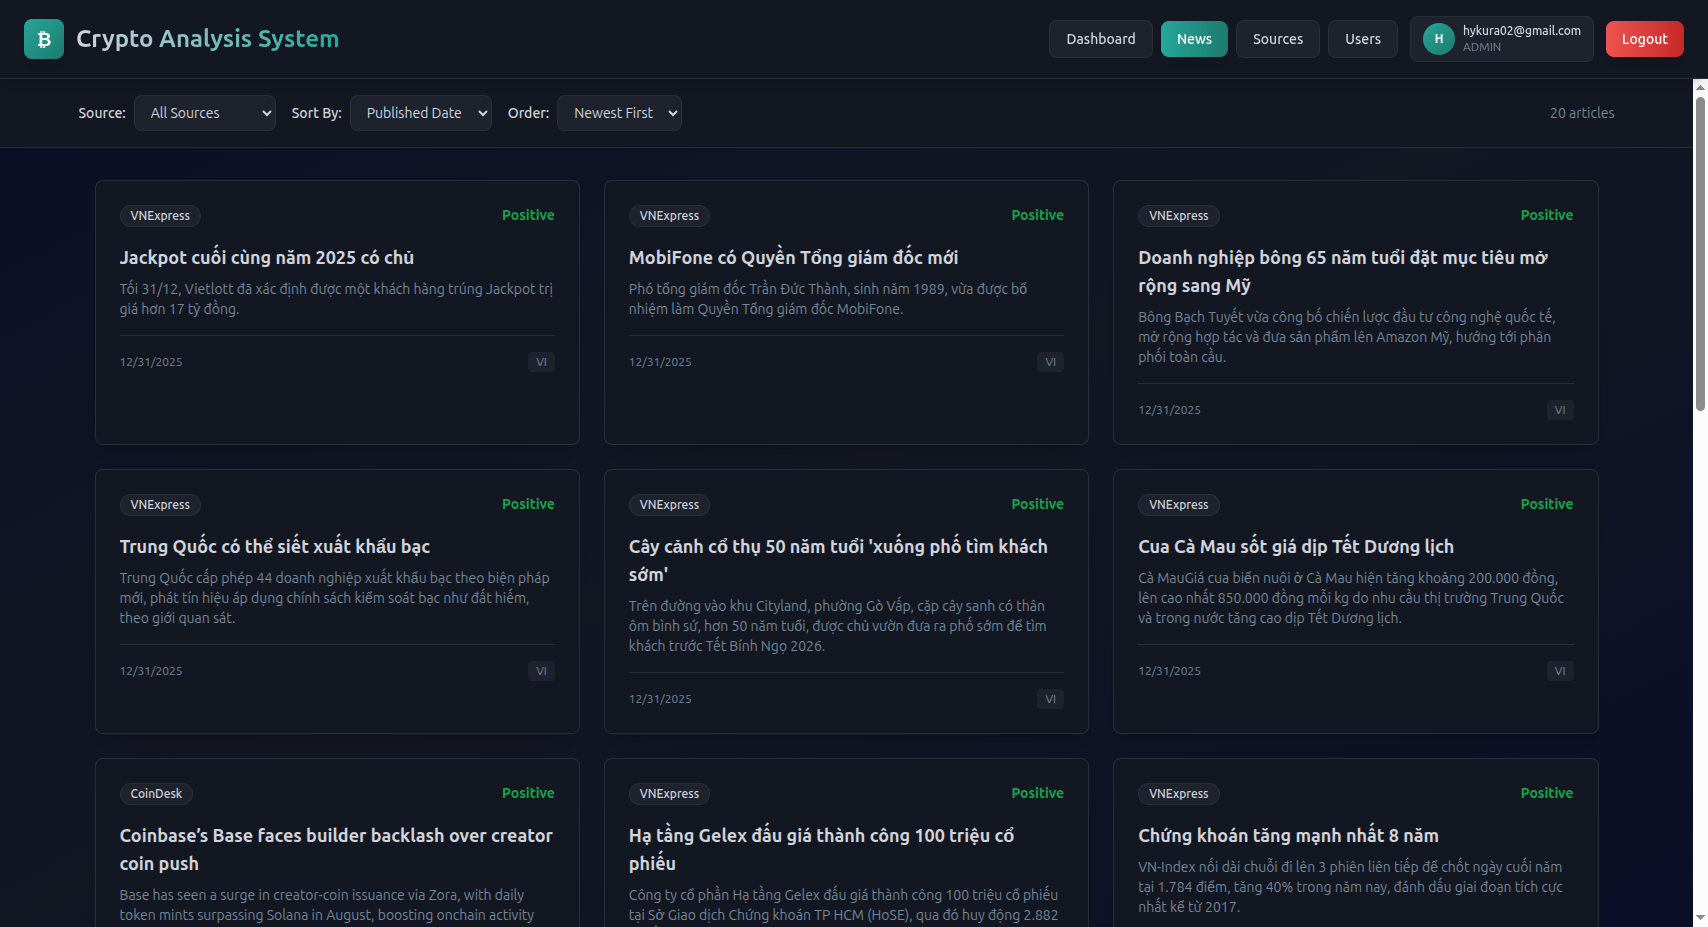
\includegraphics[width=\textwidth]{gui_news}
\caption{Giao diện News: danh sách tin tức tài chính với sentiment}
\label{fig:gui-news}
\end{figure}

\subsubsection{Login / Register}

\begin{itemize}
    \item Form đăng nhập: email, password; nút đăng nhập.
    \item Form đăng ký: email, password, first name, last name; nút đăng ký.
    \item Giao diện tối giản, tích hợp với theme tối (dark mode) của ứng dụng.
\end{itemize}

\begin{figure}[H]
\centering
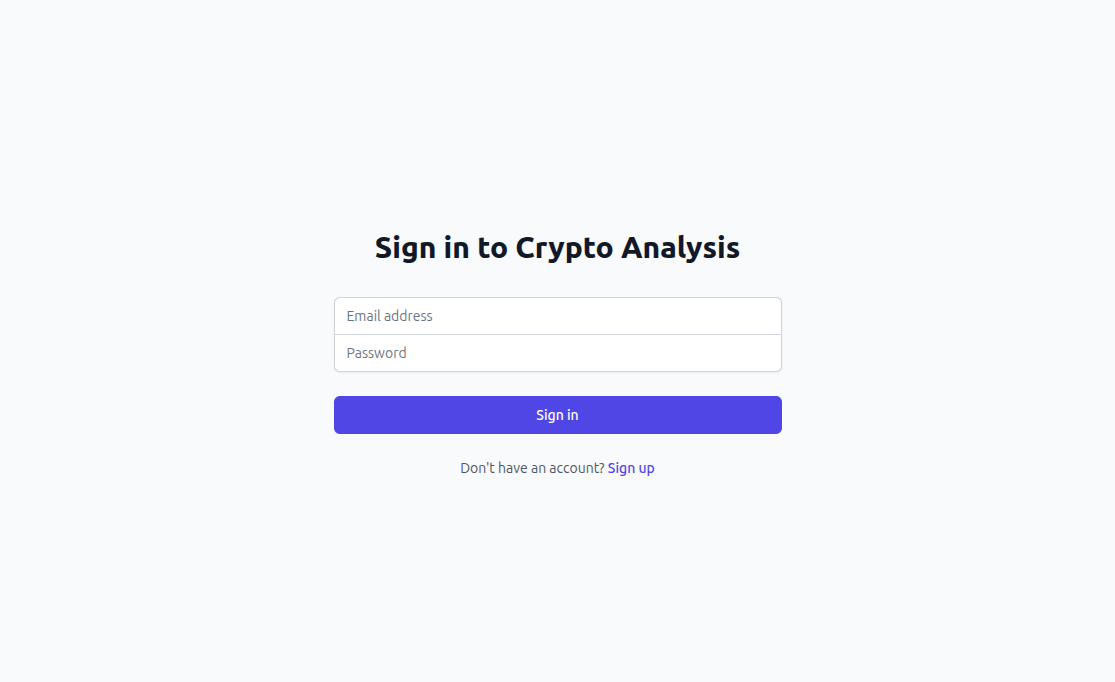
\includegraphics[width=0.7\textwidth]{gui_login}
\caption{Giao diện đăng nhập}
\label{fig:gui-login}
\end{figure}

\subsubsection{Sources (Admin)}

\begin{itemize}
    \item Bảng danh sách nguồn: source\_id, rss\_url, các selector (title\_tag, link\_tag, content\_selector, v.v.).
    \item Nút thêm/sửa/xóa; nút \textit{Analyze} để gọi Gemini AI và cập nhật selectors.
\end{itemize}

\begin{figure}[H]
\centering
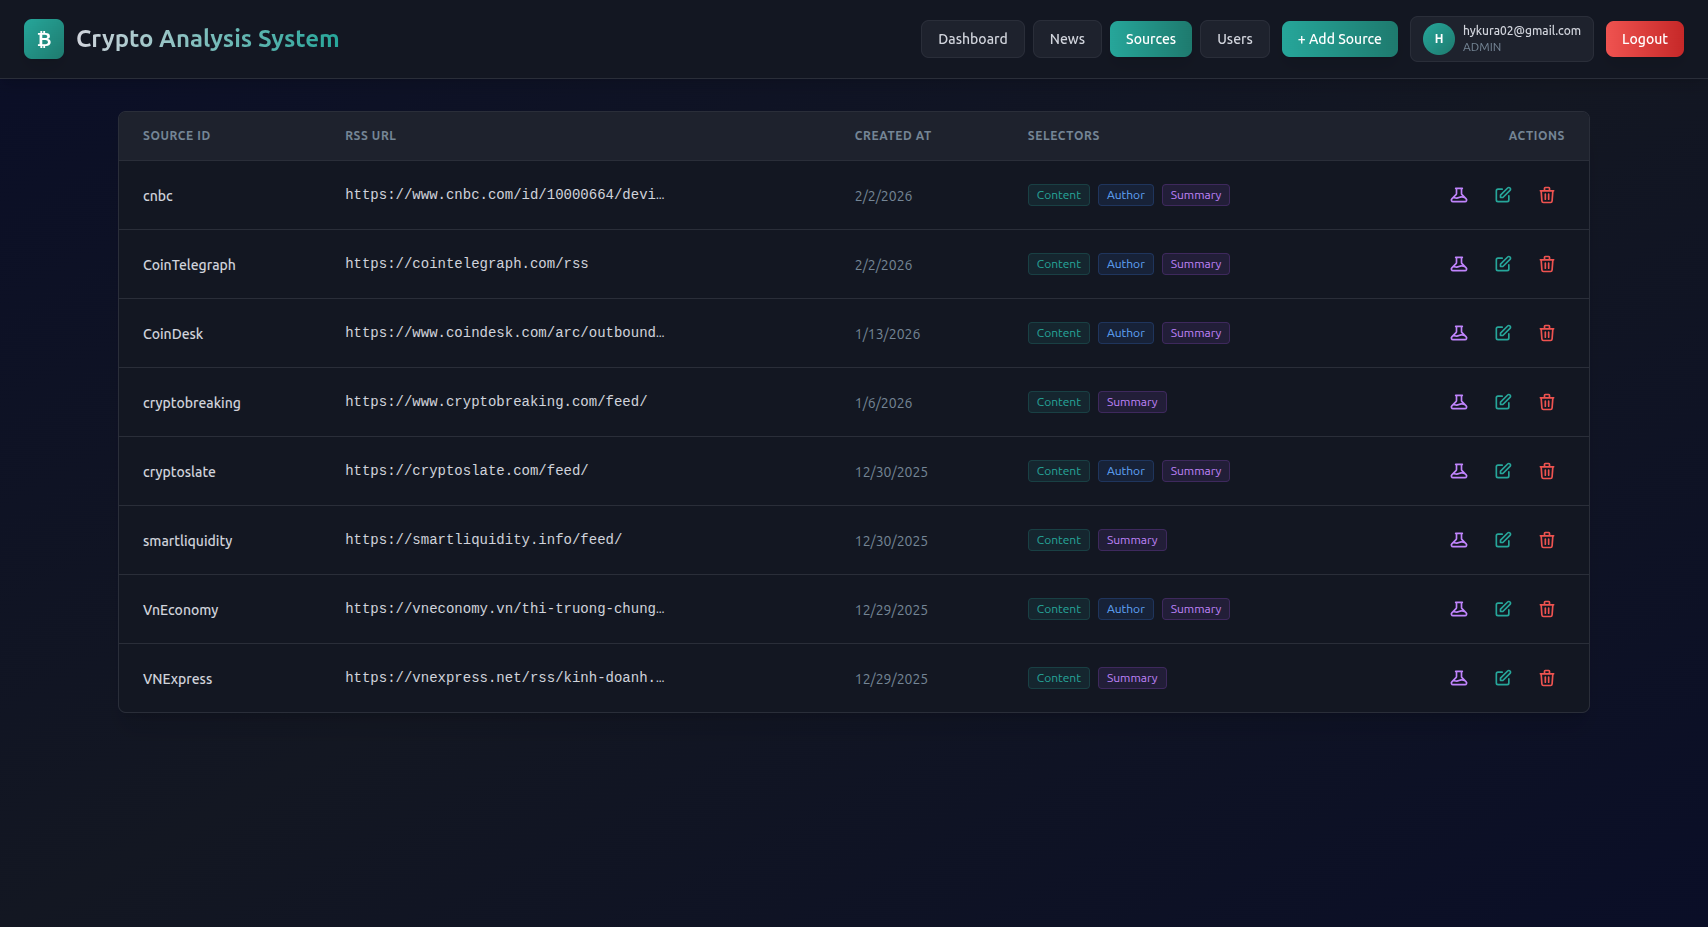
\includegraphics[width=\textwidth]{gui_sources}
\caption{Giao diện quản lý nguồn tin (Admin)}
\label{fig:gui-sources}
\end{figure}

\subsubsection{Users (Admin)}

\begin{itemize}
    \item Bảng danh sách users: USER, EMAIL, ROLE, ACTIONS.
    \item Legend role: Admin (tím), VIP (cam), Normal (xám).
    \item Dropdown đổi role cho user khác; Admin hiện tại được bảo vệ (\textit{Protected}).
\end{itemize}

\begin{figure}[H]
\centering
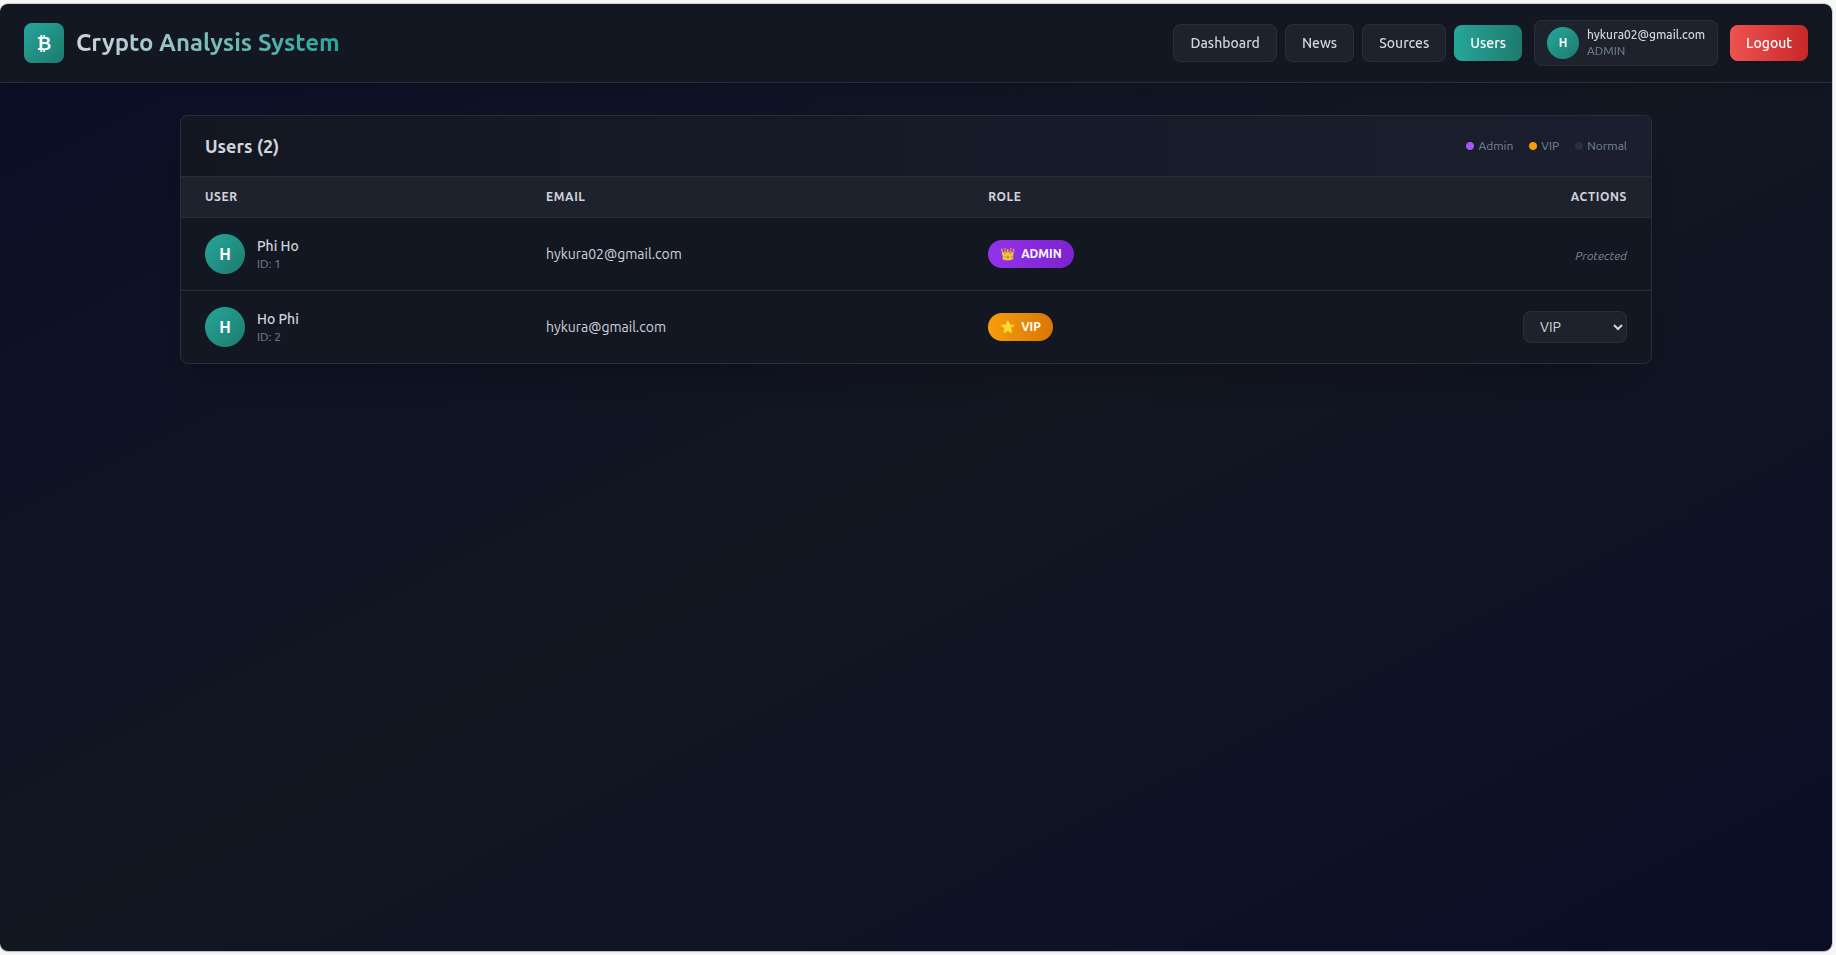
\includegraphics[width=\textwidth]{gui_users_mng}
\caption{Giao diện quản lý người dùng (Admin)}
\label{fig:gui-users}
\end{figure}

\subsection{Công nghệ giao diện}

\begin{itemize}
    \item \textbf{React + TypeScript + Vite}: Frontend SPA hiện đại.
    \item \textbf{Tailwind CSS}: Utility-first styling, responsive design.
    \item \textbf{TradingView Lightweight Charts}: Biểu đồ nến chuyên nghiệp.
    \item \textbf{TanStack Router}: Client-side routing.
    \item \textbf{Context API}: AuthContext (user, token, role), WebSocketContext (connection, subscribe).
\end{itemize}
   % Phần ứng dụng (tính năng, GUI)
% =============================================================================
% CÁC PHẦN NÂNG CAO KHÁC
% =============================================================================

\section{Các phần nâng cao khác}
\label{sec:nang-cao}

Phần này tóm tắt các tình huống kỹ thuật chính và giải pháp đã triển khai trong đồ án Crypto Analytics Platform.

\subsection{1. Xử lý Dữ liệu Thị trường Thời gian thực}

Trong hệ thống phân tích tài chính, dữ liệu giá là trái tim của nền tảng. Yêu cầu: xử lý dữ liệu real-time với độ trễ thấp, theo dõi đồng thời nhiều cặp tiền (BTC, ETH, SOL), và đảm bảo tính ổn định khi kết nối bị gián đoạn.

\textbf{Vấn đề với HTTP Polling}: (1) Lãng phí tài nguyên---phần lớn request trả về dữ liệu không đổi; (2) Độ trễ cao---luôn có độ trễ ít nhất bằng nửa chu kỳ poll; (3) Rate limit---sàn giới hạn số request (ví dụ 1200 req/phút), polling nhiều cặp tiền dễ bị chặn IP.

\textbf{Giải pháp---Market Service với WebSocket \& Event-Driven}:
\begin{itemize}
    \item \textbf{WebSocket Ingestion}: Duy trì persistent connection với Binance Stream, đăng ký stream (vd. \texttt{btcusdt@kline\_1m}), nhận push-based thay vì poll.
    \item \textbf{Hub Pattern}: Pub/Sub nội bộ fan-out dữ liệu đến nhiều đích---Frontend WebSocket, Kafka topic \texttt{market\_price\_updates}, PostgreSQL.
    \item \textbf{Tự phục hồi}: Auto-reconnect với exponential backoff (1s, 2s, 4s...); graceful degradation---nếu Kafka lỗi tạm thời, luồng WebSocket cho client vẫn hoạt động.
\end{itemize}

Luồng điển hình: Giá thay đổi $\to$ Market Service nhận event vài ms $\to$ Parse và chuẩn hóa $\to$ Phân phối song song (WebSocket clients, Kafka, DB).

\begin{figure}[H]
\centering
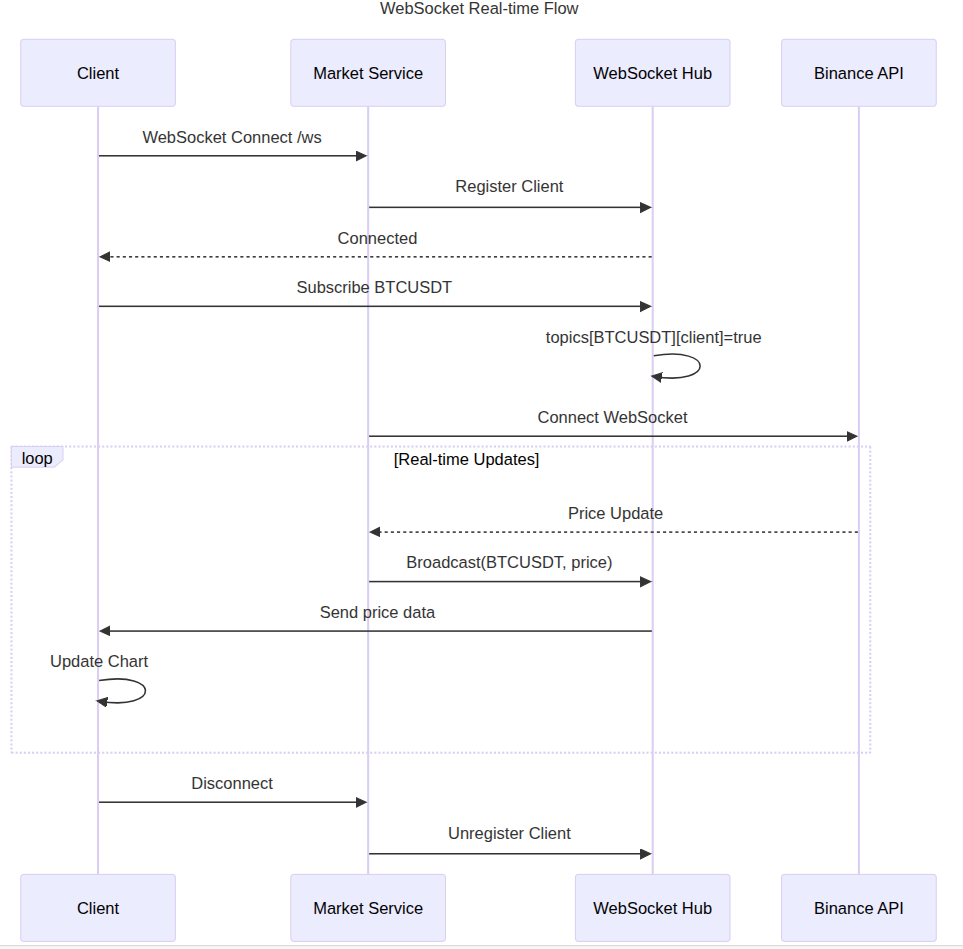
\includegraphics[width=0.9\textwidth]{sequence/sequence_websocket_flow.png}
\caption{Luồng WebSocket: Binance $\to$ Market Service $\to$ Clients}
\end{figure}

\subsection{2. Thu thập Tin tức với AI-Powered Crawler}

Cần thu thập tin tức tài chính từ hàng trăm website; nhiều trang dùng SPA (JavaScript render), cấu trúc HTML thường xuyên thay đổi. Crawler truyền thống (XPath/CSS cố định) dễ vỡ khi một class name thay đổi, chi phí bảo trì cao.

\textbf{Giải pháp---Crawler Service (Golang)}:
\begin{itemize}
    \item \textbf{RSS \& Multi-source}: Thu thập từ CoinDesk, CoinTelegraph, VNExpress, VnEconomy; goroutines crawl đồng thời.
    \item \textbf{Gemini AI CSS Selector}: Khi thêm nguồn mới, gửi HTML sample đến AI Service; Gemini (\texttt{gemini-1.5-flash}) phân tích cấu trúc và đề xuất selectors cho title, content, author, date; lưu vào DB (bảng \texttt{sources}); nếu selector fail (accuracy < 70\%), trigger re-analysis.
    \item \textbf{Kafka Event-Driven}: Bài viết mới được produce vào \texttt{news\_new\_article}; AI Service consume và phân tích sentiment; HTML cần phân tích selector vào \texttt{news\_analyze\_css\_selector}.
\end{itemize}

\textbf{Sentiment đa ngôn ngữ}: FinBERT (văn bản tài chính tiếng Anh) + PhoBERT (tiếng Việt). Pipeline: detect language $\to$ chọn model $\to$ tokenize và inference $\to$ extract attention weights cho keyword extraction. Top keywords từ attention scores cao nhất hỗ trợ người dùng hiểu nội dung chính.

\begin{figure}[H]
\centering
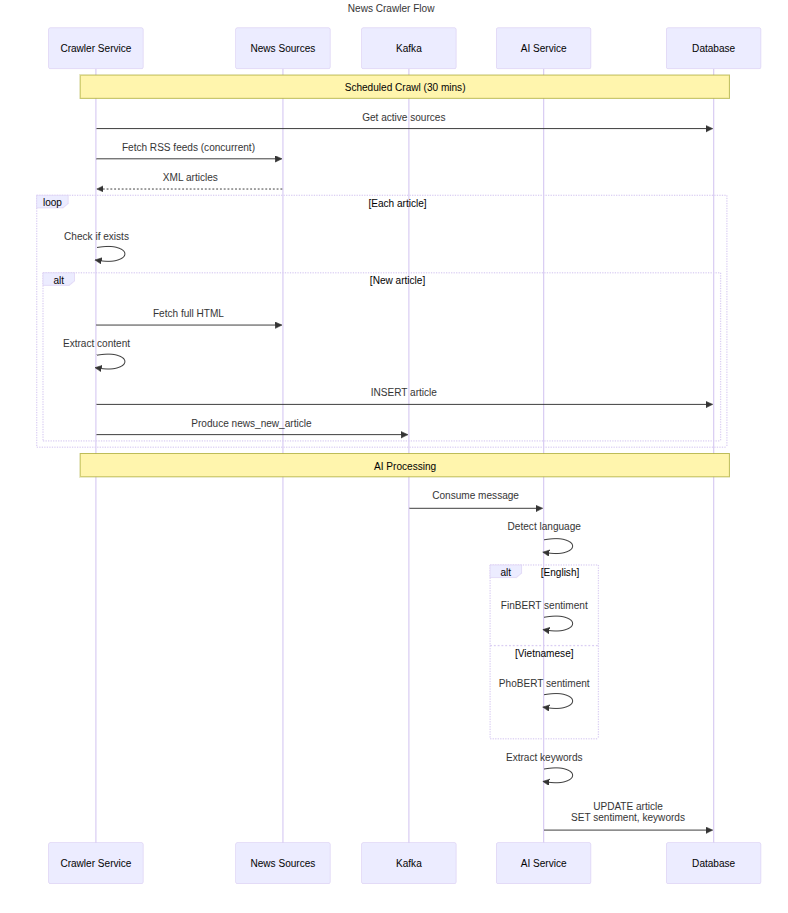
\includegraphics[width=0.9\textwidth]{sequence/sequence_crawler_flow.png}
\caption{Luồng Crawler với Kafka Event-Driven}
\end{figure}

\subsection{3. Bảo mật và Phân quyền}

Phát hiện truy cập bất thường---bypass API Gateway, JWT cũ vẫn hợp lệ, token replay. Hạn chế JWT alone: (1) Không thu hồi được sau khi cấp; (2) Thiếu Single Source of Truth; (3) Key rotation phức tạp.

\textbf{Giải pháp---Auth Service}:
\begin{itemize}
    \item \textbf{Access Token (JWT, short-lived)}: Claims \texttt{sub}, \texttt{email}, \texttt{role}, \texttt{iat}, \texttt{exp}; thời hạn 15--30 phút.
    \item \textbf{Refresh Token (opaque, lưu DB)}: Thời hạn dài hơn; lưu trong \texttt{refresh\_tokens}; mỗi lần \texttt{/auth/refresh} thành công thì rotate---vô hiệu hóa token cũ, cấp token mới.
    \item \textbf{Logout/Revoke}: Xóa refresh token trong DB; có thể blacklist JWT compromise.
    \item \textbf{Bcrypt} cho password hashing; token qua cookie \texttt{HttpOnly}, \texttt{Secure}, \texttt{SameSite}.
\end{itemize}

\textbf{Phân quyền VIP/Normal}: Middleware \texttt{RequireVIP} kiểm tra role từ JWT; tài khoản thường---xem biểu đồ, tin tức cơ bản; VIP/ADMIN---xem AI Prediction, SHAP explanation, sentiment scores, top keywords. \textbf{Zero-Trust}: API Gateway single entry point; validate mọi input; mTLS giữa services (khi triển khai Service Mesh).

\begin{figure}[H]
\centering
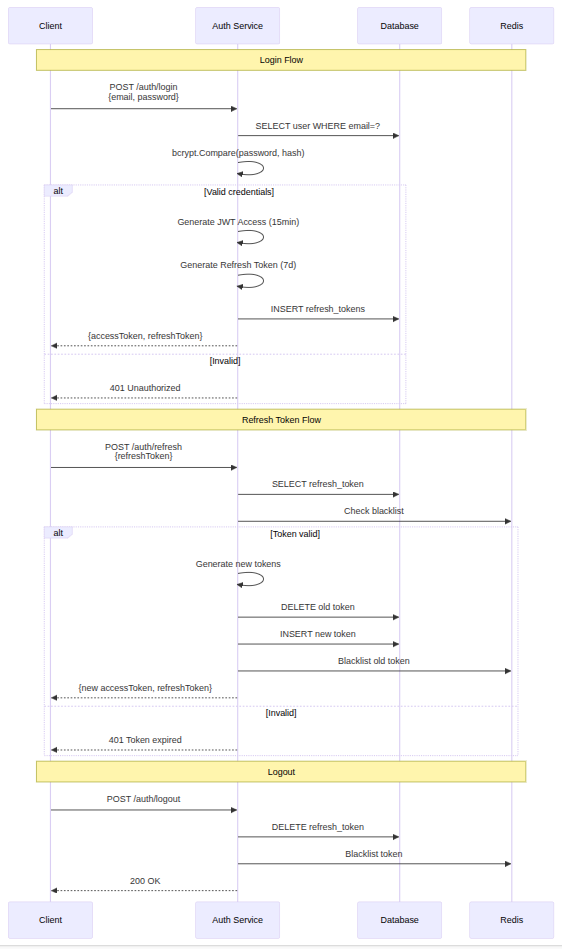
\includegraphics[width=0.85\textwidth]{sequence/sequence_auth_flow.png}
\caption{Luồng Authentication: JWT + Refresh Token}
\end{figure}

\subsection{4. Dự đoán Giá với Explainable AI (XAI)}

Yêu cầu: dự đoán xu hướng giá UP/DOWN (1h, 4h, 24h), kết hợp tin tức với giá lịch sử, và \textbf{giải thích} tại sao model đưa ra dự đoán. Black-box AI gây thiếu tin cậy, khó debug, không đạt chuẩn regulatory.

\textbf{Pipeline---XGBoost + SHAP}:
\begin{itemize}
    \item \textbf{Technical Features}: RSI, MACD, SMA, returns (\texttt{return\_1h}, \texttt{return\_24h}), volatility, lag features (\texttt{close\_lag\_1}, \texttt{close\_lag\_24}).
    \item \textbf{News Features}: Time-align tin tức với price theo hourly buckets; \texttt{sentiment\_mean}, \texttt{news\_count}, \texttt{sentiment\_ma\_24h}, \texttt{sentiment\_lag\_1h/6h}; merge left join, fill missing = 0.
    \item \textbf{Model}: XGBoost Regressor (200 trees, max\_depth=6, learning\_rate=0.05); train/test split 80/20 chronologically; target = future price sau \texttt{horizon\_hours}.
    \item \textbf{SHAP TreeExplainer}: Tính contribution từng feature; sort theo |SHAP|; top 10 features + phân loại news vs technical; \texttt{news\_influence\_pct} để người dùng thấy mức độ ảnh hưởng của tin tức.
\end{itemize}

\textbf{Top News \& Confidence}: Top 3 bài viết trong lookback window; keywords từ attention weights. Confidence = trung bình có trọng số của feature coverage, news availability, balance score (tỷ lệ news features gần 30\%).

\begin{figure}[H]
\centering
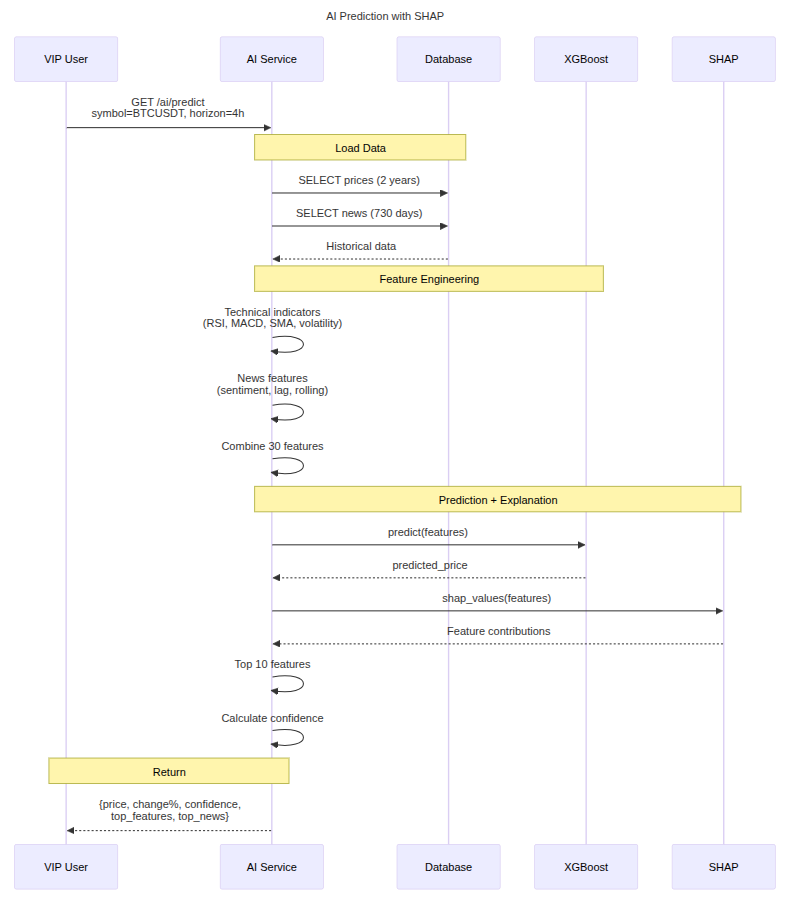
\includegraphics[width=0.9\textwidth]{sequence/sequence_ai_prediction_flow.png}
\caption{Luồng AI Prediction với SHAP XAI}
\end{figure}

\subsection{5. Topic-based WebSocket Hub}

Khi nhiều người dùng đồng thời kết nối WebSocket, cần cơ chế broadcast hiệu quả. Hub dùng \textbf{topic-based subscription}: mỗi client subscribe các topics (vd. \texttt{btcusdt@kline\_1m}, \texttt{ethusdt@kline\_5m}); server chỉ broadcast đến clients đã subscribe topic tương ứng, tránh gửi dữ liệu không liên quan.

\textbf{Mở rộng đa server}: (1) \textbf{Kafka}---mỗi Market instance publish vào topic; consumer redistribute đến WebSocket clients; (2) \textbf{Redis Pub/Sub}---các Hub instances subscribe channel; instance nhận dữ liệu publish lên Redis; instances khác nhận và broadcast local; (3) \textbf{Sticky Session}---Load balancer giữ client với cùng Market instance cho một symbol. Hệ thống hiện có Kafka producer \texttt{market\_price\_update} sẵn sàng cho mở rộng.

\begin{figure}[H]
\centering
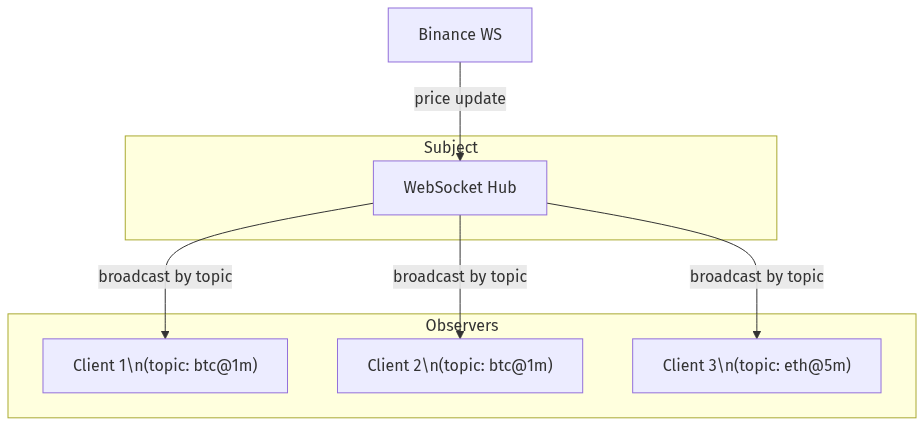
\includegraphics[width=0.85\textwidth]{pattern_observer}
\caption{Topic-based WebSocket Hub}
\label{fig:nangcao-websocket}
\end{figure}

\subsection{6. Gemini AI CSS Selector \& Multi-language Sentiment}

\textbf{Gemini AI}: Workflow---Crawler gửi HTML sample qua Kafka topic \texttt{news\_analyze\_css\_selector}; AI Service gọi \texttt{gemini-1.5-flash} với prompt mô tả cấu trúc trang; model đề xuất CSS selectors cho title, link, content, author; validate và lưu vào bảng \texttt{sources}; lần crawl sau dùng selectors đã học. Khi website đổi layout, admin gọi \textit{Analyze} lại mà không cần sửa code.

\textbf{FinBERT + PhoBERT}: Tin tức có cả tiếng Anh và tiếng Việt. FinBERT (\texttt{yiyanghkust/finbert-tone}) chuyên văn bản tài chính en; PhoBERT (\texttt{wonrax/phobert-base-vietnamese-sentiment}) cho vi. Pipeline: langdetect $\to$ chọn model $\to$ tokenize (underthesea cho vi) $\to$ inference. Strategy pattern cho phép dễ thêm model mới.

\begin{figure}[H]
\centering
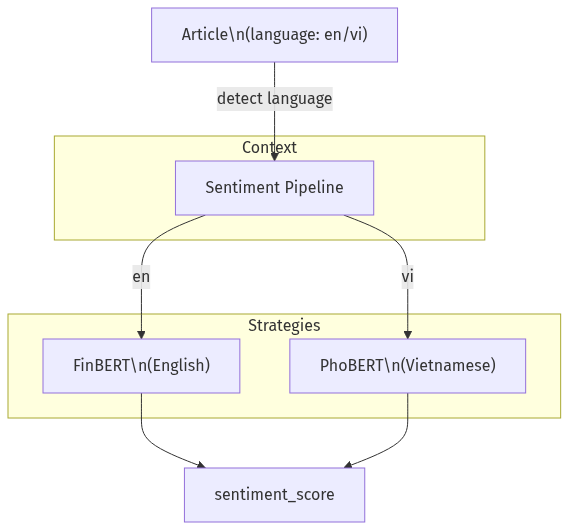
\includegraphics[width=0.75\textwidth]{pattern_strategy}
\caption{Strategy: FinBERT / PhoBERT}
\label{fig:nangcao-sentiment}
\end{figure}

\subsection{7. Event-driven với Kafka}

Các service giao tiếp qua Kafka topics: \texttt{news\_new\_article} (Crawler $\to$ AI), \texttt{news\_analyze\_css\_selector} (Crawler $\to$ AI cho HTML analysis), \texttt{market\_price\_update} (Market $\to$ AI/consumers). Lợi ích: \textbf{loose coupling}---Crawler và AI chạy bất đồng bộ; AI chậm không block Crawler; \textbf{scalability}---dễ thêm consumer mới (vd. notification service) mà không sửa Crawler; \textbf{reliability}---Kafka đảm bảo message delivery, có thể replay khi consumer fail.

\subsection{Tổng kết giải pháp}

\begin{table}[H]
\centering
\caption{Tóm tắt giải pháp kỹ thuật}
\begin{tabular}{|l|l|l|}
\hline
\textbf{Tình huống} & \textbf{Vấn đề} & \textbf{Giải pháp} \\
\hline
WebSocket Scale & Polling tốn tài nguyên & Hub + Topic-based + Kafka \\
\hline
Crawler & HTML thay đổi & Gemini AI selector, RSS \\
\hline
Security & JWT không revoke được & Refresh Token + DB \\
\hline
AI Prediction & Black-box & XGBoost + SHAP XAI \\
\hline
Multi-language & en/vi & FinBERT + PhoBERT \\
\hline
\end{tabular}
\end{table}
   % Các phần nâng cao khác (đã gộp nội dung ch 1,2,3,5,ai)
% =============================================================================
% KẾT LUẬN VÀ ĐÁNH GIÁ
% =============================================================================

\section{Kết luận và Đánh giá}
\label{sec:ket-luan-danh-gia}

\subsection{Đánh giá hiệu quả kiến trúc và thay đổi đã thực hiện}

\subsubsection{Kiến trúc Microservices}

Kiến trúc microservices với event-driven (Kafka) đã chứng minh hiệu quả:
\begin{itemize}
    \item \textbf{Tách biệt trách nhiệm}: Auth, Market, Crawler, AI mỗi service một nhiệm vụ rõ ràng; sửa lỗi hoặc nâng cấp một service không ảnh hưởng các service khác.
    \item \textbf{Scale độc lập}: Có thể scale Market Service (WebSocket) và Crawler Service theo nhu cầu tải khác nhau.
    \item \textbf{Công nghệ đa dạng}: Golang cho real-time và crawler; Python cho AI/ML; React cho frontend --- mỗi layer dùng công nghệ phù hợp.
\end{itemize}

\subsubsection{Thay đổi và cải tiến đã thực hiện}

\begin{itemize}
    \item \textbf{WebSocket Hub với Topic-based subscription}: Thay vì broadcast toàn bộ, mỗi client chỉ nhận dữ liệu cho symbol/timeframe đã subscribe --- giảm tải mạng và CPU.
    \item \textbf{Gemini AI cho CSS Selector}: Giảm công sức bảo trì khi website nguồn tin thay đổi layout.
    \item \textbf{Explainable AI (SHAP)}: Tăng độ tin cậy của dự đoán; người dùng hiểu lý do model đưa ra kết quả.
    \item \textbf{Redis Cache cho Prediction}: Giảm gọi AI Service lặp lại; cải thiện thời gian phản hồi cho người dùng VIP.
\end{itemize}

\subsection{Bài học kinh nghiệm}

\begin{enumerate}
    \item \textbf{Thiết kế chấp nhận lỗi}: Mọi service trong hệ thống phân tán đều có thể fail. Cần có fallback (ví dụ: AI Service down thì ẩn Prediction Panel, vẫn hiển thị biểu đồ và tin tức).
    
    \item \textbf{Stateless và external state}: Services stateless dễ scale; state lưu ở PostgreSQL và Redis thay vì trong memory.
    
    \item \textbf{Security by Design}: JWT + Refresh Token, role-based middleware, không tin input từ client --- validate và sanitize mọi nơi.
    
    \item \textbf{Observability}: Logging, metrics, tracing là cần thiết; khi triển khai production nên bổ sung Prometheus, Grafana, centralized logging.
    
    \item \textbf{Documentation và contracts}: API contracts (OpenAPI), schema DBML, mermaid diagrams giúp onboarding và bảo trì dễ dàng hơn.
\end{enumerate}

\subsection{Đề xuất cải tiến và phát triển tương lai}

Dựa trên kinh nghiệm thu được (chi tiết hơn xem phần Kết luận và Bài học rút ra):
\begin{itemize}
    \item \textbf{Kubernetes}: Migrate từ Docker Compose sang K8s; HPA cho auto-scaling; multi-AZ cho high availability.
    \item \textbf{Service Mesh}: Istio/Linkerd cho mTLS, traffic management, distributed tracing tự động.
    \item \textbf{Advanced ML}: Thử LSTM/Transformer cho time-series; online learning; A/B testing models.
    \item \textbf{CI/CD}: GitHub Actions cho automated test và deploy; blue-green deployment.
    \item \textbf{Read Replicas}: PostgreSQL replication cho read-heavy workloads (list articles, validate token).
\end{itemize}

\subsection{Thuận lợi và khó khăn khi làm đồ án}

\subsubsection{Thuận lợi}

\begin{itemize}
    \item \textbf{Công nghệ sẵn có}: Golang, Python, React, PostgreSQL, Kafka, Redis đều có tài liệu phong phú và cộng đồng lớn.
    \item \textbf{Binance API}: REST và WebSocket miễn phí, documentation rõ ràng; dễ tích hợp dữ liệu giá real-time.
    \item \textbf{HuggingFace}: FinBERT, PhoBERT pre-trained sẵn; giảm thời gian train model sentiment.
    \item \textbf{Docker Compose}: Triển khai toàn bộ stack (Postgres, Redis, Kafka, services) trên máy local một lệnh; dễ phát triển và demo.
\end{itemize}

\subsubsection{Khó khăn}

\begin{itemize}
    \item \textbf{Đồng bộ time-series}: Align tin tức với giá theo time buckets (process\_news) phức tạp; phải xử lý timezone, định dạng ngày tháng khác nhau từ các nguồn.
    \item \textbf{HTML thay đổi}: Các trang tin tức thường đổi layout; giải pháp Gemini AI giúp giảm công bảo trì nhưng vẫn cần kiểm tra định kỳ.
    \item \textbf{Scale WebSocket}: Một Hub instance có giới hạn connections; khi cần scale đa server phải thiết kế lại (Kafka, Redis Pub/Sub).
    \item \textbf{Chi phí AI}: Gemini API và models HuggingFace tốn tài nguyên; cần cache (Redis) và tối ưu gọi API.
\end{itemize}
 % Kết luận và Đánh giá
    % =============================================================================
    % TÀI LIỆU THAM KHẢO
    % =============================================================================

    \section*{TÀI LIỆU THAM KHẢO}
    \addcontentsline{toc}{section}{Tài liệu tham khảo}

    \begin{enumerate}
        \item \href{https://medium.com/lumen-engineering-blog/how-to-implement-a-distributed-and-auto-scalable-websocket-server-architecture-on-kubernetes-4cc32e1dfa45}{How to implement a distributed and auto scalable WebSocket server architecture on Kubernetes}. Medium - Lumen Engineering Blog.
        
        \item \href{https://www.uber.com/blog/omphalos/}{Omphalos, Uber's Parallel and Language-Extensible Time Series Backtesting Tool}. Uber Engineering Blog.
        
        \item \href{https://frontegg.com/blog/oauth-vs-jwt}{OAuth vs. JWT: What Is the Difference \& Using Them Together}. Frontegg.
        
        \item \href{https://strapi.io/blog/jwt-vs-oauth}{JWT vs OAuth: Build a Future-Proof Authentication System}. Strapi.
        
        \item \href{https://medium.com/@abhishek4023/the-growing-importance-of-a-separate-authorization-service-in-modern-microservices-architectures-58a2917f866c}{The Growing Importance of a Separate Authorization Service in Modern Microservices Architectures}. Medium.
        
        \item \href{https://www.osohq.com/post/microservices-authorization-patterns}{Best Practices for Authorization in Microservices}. Oso.
        
        \item \href{https://medium.com/hexaworks-papers/managing-user-authentication-and-authorization-in-microservices-architectures-fae705f40627}{Managing User Authentication and Authorization in Microservices Architectures}. Medium - Hexaworks Papers.
        
        \item \href{https://pkg.go.dev/github.com/gorilla/websocket}{Gorilla WebSocket Documentation}.
        
        \item \href{https://github.com/cjhutto/vaderSentiment}{VADER Sentiment Analysis}. GitHub.
        
        \item \href{https://www.crummy.com/software/BeautifulSoup/}{Beautiful Soup Documentation}.
        
        \item \href{https://binance-docs.github.io/apidocs/spot/en/}{Binance API Documentation}.
        
        \item \href{https://gin-gonic.com/docs/}{Gin Web Framework Documentation}.
        
        \item \href{https://docs.docker.com/compose/}{Docker Compose Documentation}.
        
        \item \href{https://www.postgresql.org/docs/}{PostgreSQL Documentation}.
        
        \item \href{https://redis.io/documentation}{Redis Documentation}.
    \end{enumerate}


\end{document}
